% !TeX program = lualatex
\documentclass[11pt,a4paper]{article}
\usepackage{szzmaterial}
\usetikzlibrary{calc,positioning,arrows.meta,fit}
\setlist[enumerate]{nosep,leftmargin=2.1em}
\setlist[itemize]{nosep,leftmargin=1.8em}

% --- Lokální makra okruhu ---
\newcommand{\Mset}{\mathrm{M}}              % třída modelů
\newcommand{\Csq}{\operatorname{Csq}}       % důsledky teorie
\newcommand{\Th}{\operatorname{Th}}         % teorie struktury
\newcommand{\Var}{\operatorname{Var}}
% Prázdná klauzule (\conn chybí v Libertinus -- kreslíme rámeček):
\newcommand{\eclause}{\mathord{\text{\framebox[1.25ex][c]{\rule{0pt}{0.95ex}}}}}
% Zástupný symbol pro obecnou binární spojku (\conn v Libertinus chybí):
\newcommand{\conn}{\mathbin{\vcenter{\hbox{\framebox[1.05ex][c]{\rule{0pt}{0.72ex}}}}}}
% Značky větví tabla:
\newcommand{\closed}{\ensuremath{\otimes}}            % sporná větev
\newcommand{\open}{\textcolor{green!45!black}{\faCheck}} % dokončená bezesporná

\szztitul{Logika}{M6}{NAIL062 (Výroková a predikátová logika)}

\begin{document}
\maketitle
\tableofcontents
\bigskip

\section*{Úvod}
\addcontentsline{toc}{section}{Úvod}

Tento materiál pokrývá okruh \textbf{M6 -- Logika} (předmět NAIL062 \emph{Výroková a predikátová logika}). Výklad stojí na \textbf{skriptech přednášejícího dr.~Jakuba Bulína} (\emph{NAIL062 Výroková a predikátová logika: zápisky z přednášky}, zimní semestr 2025), jejichž struktura i obsah jsou převzaty z dřívějších přednášek P.~Gregora a z učebnic A.~Nerode, R.~Shore \emph{Logic for Applications} a M.~Ben-Ari \emph{Mathematical Logic for Computer Science}. Značení a hloubka odpovídají kurzu pro informatiky.

Logika má dvě patra: \textbf{výrokovou logiku} (atomy jsou nedělitelné \uv{prvovýroky} bez vnitřní struktury) a \textbf{predikátovou logiku prvního řádu} (atomy mluví o individuích pomocí relací, funkcí a kvantifikátorů). Obě patra procházíme paralelně ve čtyřech vrstvách: \emph{syntaxe} (jak vypadají formule), \emph{sémantika} (co znamenají, kdy platí), \emph{dokazatelnost} (jak platnost ověřit syntaktickým výpočtem) a \emph{metavěty} (korektnost, úplnost, kompaktnost, rozhodnutelnost), které obě vrstvy spojují.

\medskip
\noindent\textbf{Role důkazů.} Požadavky okruhu výslovně žádají \textbf{schopnost vést formální důkaz} v~některém dokazovacím systému (tablo metoda, rezoluce, Hilbertovský kalkul), kdežto u~vět o~kompaktnosti a~úplnosti jen \emph{znění, porozumění významu a~použití}. Tablo a~rezoluční postupy proto rozepisujeme do detailu (krok po kroku, celé stromy), zatímco metavěty komentujeme intuicí, náčrtem myšlenky a~aplikacemi. Do výkladu je zařazena řešená reálná otázka SZZ k~okruhu (léto 2024: model teorie); je i v~samostatném dokumentu \emph{Příklady otázek}. Použité zdroje jsou uvedeny na konci.

\medskip
\noindent\textbf{Značení.} Prvovýroky (výrokové proměnné) značíme $p,q,r$, výrokové formule řeckými písmeny $\varphi,\psi,\chi$; binární spojku zastupuje $\conn\in\{\wedge,\vee,\to,\leftrightarrow\}$. Teorie je množina formulí $T$, její prvky jsou \emph{axiomy}. V predikátové logice je \emph{signatura} $\langle\mathcal R,\mathcal F\rangle$ (relační a funkční symboly s aritami; konstanty jsou nulární funkce), \emph{struktura} $\mathcal A=\langle A,\mathcal R^{\mathcal A},\mathcal F^{\mathcal A}\rangle$ s neprázdnou doménou $A$. Sémantické vyplývání (platnost) píšeme $\models$, syntaktickou dokazatelnost $\vdash$. Třídu modelů teorie $T$ značíme $\Mset(T)$, množinu důsledků $\Csq(T)$, teorii struktury $\Th(\mathcal A)$. Prázdná klauzule je $\eclause$. Sjednocujeme značení s okruhy M2 (algebraické struktury), M3 (relace, ekvivalence) a M4 (grafy jako struktury), na něž místy odkazujeme.

% ============================================================
\section{Syntaxe a normální formy (CNF, DNF, PNF)}

Syntaxe popisuje, \emph{jak formule vypadají} -- jako konečné nápisy vzniklé podle gramatických pravidel, bez ohledu na význam. Klíčová je induktivní definice a stromová struktura, díky níž je každá formule jednoznačně čitelná.

\subsection{Jazyk a formule výrokové logiky}

\begin{definice}[Jazyk a výrok]
\emph{Jazyk} výrokové logiky je neprázdná množina $\mathbb{P}$ \emph{prvovýroků} (výrokových proměnných), obvykle spočetná. \emph{Výrok (výroková formule)} v~jazyce $\mathbb{P}$ je prvek nejmenší množiny $\mathrm{VF}_{\mathbb{P}}$ takové, že
\begin{enumerate}[label=(\arabic*)]
  \item každý prvovýrok $p\in\mathbb{P}$ je výrok;
  \item je-li $\varphi$ výrok, je výrokem i $(\neg\varphi)$;
  \item jsou-li $\varphi,\psi$ výroky, je výrokem i $(\varphi\conn\psi)$ pro $\conn\in\{\wedge,\vee,\to,\leftrightarrow\}$.
\end{enumerate}
\emph{Podvýrok} je podřetězec, který je sám výrokem. \emph{Teorie} je libovolná množina výroků $T\subseteq\mathrm{VF}_{\mathbb{P}}$.
\end{definice}

\begin{intuice}
Definice je \emph{induktivní}: výroky jsou přesně ty konečné nápisy, které vzniknou konečně mnoha aplikacemi pravidel z prvovýroků. Vnější závorky a méně závorek píšeme dle priority $\neg$ (nejvyšší) $>\ \wedge,\vee\ >\ \to,\leftrightarrow$ (nejnižší); $\wedge,\vee$ asociují doprava. Tatáž data lze zapsat prefixově (polsky) i postfixově -- podstatná je stromová struktura, ne řetězec znaků.
\end{intuice}

\begin{definice}[Strom výroku]
\emph{Strom výroku} $\mathrm{Tree}(\varphi)$ je zakořeněný uspořádaný strom: prvovýrok $p$ má jediný vrchol s~návěštím $p$; výrok $(\neg\varphi')$ má kořen $\neg$ s~jediným synem $\mathrm{Tree}(\varphi')$; výrok $(\varphi'\conn\psi')$ má kořen $\conn$ s~levým synem $\mathrm{Tree}(\varphi')$ a~pravým $\mathrm{Tree}(\psi')$. Podstromy odpovídají podvýrokům.
\end{definice}

\begin{center}
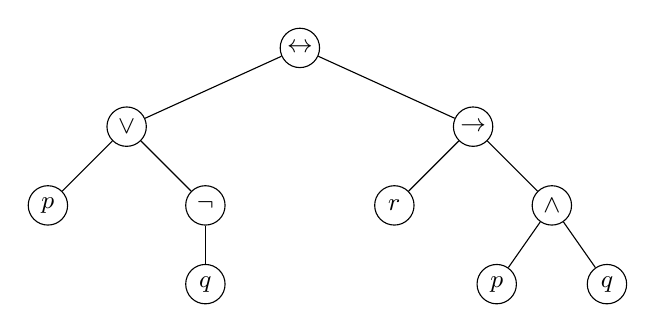
\begin{tikzpicture}[scale=1.0,level distance=10mm,
  every node/.style={font=\small},
  lbl/.style={circle,draw,inner sep=1.6pt,minimum size=5mm}]
  \node[lbl] (root) at (0,0) {$\leftrightarrow$};
  \node[lbl] (l) at (-2.2,-1) {$\vee$};
  \node[lbl] (r) at (2.2,-1) {$\to$};
  \node[lbl] (lp) at (-3.2,-2) {$p$};
  \node[lbl] (lneg) at (-1.2,-2) {$\neg$};
  \node[lbl] (lnegq) at (-1.2,-3) {$q$};
  \node[lbl] (rr) at (1.2,-2) {$r$};
  \node[lbl] (rand) at (3.2,-2) {$\wedge$};
  \node[lbl] (randp) at (2.5,-3) {$p$};
  \node[lbl] (randq) at (3.9,-3) {$q$};
  \draw (root)--(l); \draw (root)--(r);
  \draw (l)--(lp); \draw (l)--(lneg); \draw (lneg)--(lnegq);
  \draw (r)--(rr); \draw (r)--(rand); \draw (rand)--(randp); \draw (rand)--(randq);
\end{tikzpicture}\obrpopis{Strom výroku $\varphi=\big((p\vee\neg q)\leftrightarrow(r\to(p\wedge q))\big)$. Kořen je hlavní spojka $\leftrightarrow$, listy jsou prvovýroky; $\Var(\varphi)=\{p,q,r\}$. Každý podvýrok je podstrom.}
\end{center}

\subsection{Jazyk a formule predikátové logiky}

Výroková logika nevidí dovnitř atomů. Predikátová logika \emph{prvního řádu} mluví o~\emph{individuích} (prvcích nějaké domény): vyjadřuje jejich vlastnosti a vztahy (relace), skládá je funkcemi a kvantifikuje přes \uv{všechna} ($\forall$) a \uv{nějaké} ($\exists$) individuum.

\begin{definice}[Jazyk, termy, formule]
\emph{Jazyk} predikátové logiky je dán \emph{signaturou} $\langle\mathcal R,\mathcal F\rangle$ (disjunktní množiny relačních a funkčních symbolů s~aritami; konstantní symbol je funkční symbol arity~$0$) a údajem, zda jde o~\emph{jazyk s~rovností} (smí se užívat predikát $=$). K~dispozici jsou navíc spočetně mnoho \emph{proměnných} $x,y,z,\dots$, spojky, závorky a~kvantifikátory $(\forall x),(\exists x)$.
\begin{itemize}
  \item \emph{Termy:} každá proměnná a~každý konstantní symbol je term; je-li $f\in\mathcal F$ arity $n$ a~$t_1,\dots,t_n$ termy, je termem i~$f(t_1,\dots,t_n)$.
  \item \emph{Atomická formule:} $R(t_1,\dots,t_n)$ pro $n$-ární $R\in\mathcal R$ (či $=$), $t_i$ termy.
  \item \emph{Formule:} každá atomická formule je formule; jsou-li $\varphi,\psi$ formule, jsou jimi i~$(\neg\varphi)$, $(\varphi\conn\psi)$; je-li $\varphi$ formule a~$x$ proměnná, jsou formulemi i~$((\forall x)\varphi)$ a~$((\exists x)\varphi)$.
\end{itemize}
\end{definice}

\begin{intuice}
Termy jsou \uv{jména prvků} (vyhodnotí se na prvek domény), formule mají pravdivostní hodnotu. Term i~formuli zachycuje \emph{strom} (vnitřní vrcholy = funkční/relační symboly a~spojky, kvantifikátor má jako $\neg$ jediného syna). Pozor: termy jsou čistě syntaktické -- $1+1$ je term v~jazyce aritmetiky, ale jeho \uv{hodnota} $2$ termem není.
\end{intuice}

\begin{center}
\begin{minipage}[t]{0.46\linewidth}\centering
{\small (a) strom termu $(S(0)+x)\cdot y$}\\[2mm]
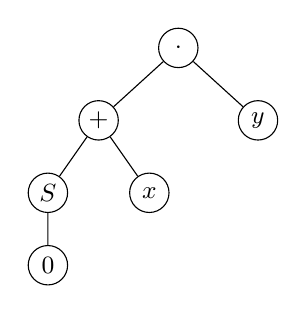
\begin{tikzpicture}[scale=0.92,level distance=9mm,every node/.style={font=\small},
  lbl/.style={circle,draw,inner sep=1.5pt,minimum size=5mm}]
  \node[lbl] (m) at (0,0) {$\cdot$};
  \node[lbl] (pl) at (-1.1,-1) {$+$};
  \node[lbl] (y) at (1.1,-1) {$y$};
  \node[lbl] (s) at (-1.8,-2) {$S$};
  \node[lbl] (x) at (-0.4,-2) {$x$};
  \node[lbl] (z) at (-1.8,-3) {$0$};
  \draw (m)--(pl); \draw (m)--(y); \draw (pl)--(s); \draw (pl)--(x); \draw (s)--(z);
\end{tikzpicture}
\end{minipage}\hfill
\begin{minipage}[t]{0.46\linewidth}\centering
{\small (b) strom formule $(\forall x)\big(x\cdot y\le(S(0)+x)\cdot y\big)$}\\[2mm]
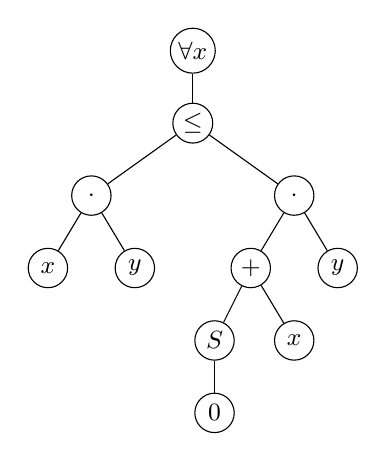
\begin{tikzpicture}[scale=0.92,level distance=9mm,every node/.style={font=\small},
  lbl/.style={circle,draw,inner sep=1.5pt,minimum size=5mm}]
  \node[lbl] (q) at (0,0.0) {$\forall x$};
  \node[lbl] (le) at (0,-1) {$\le$};
  \node[lbl] (ml) at (-1.4,-2) {$\cdot$};
  \node[lbl] (mr) at (1.4,-2) {$\cdot$};
  \node[lbl] (lx) at (-2.0,-3) {$x$};
  \node[lbl] (ly) at (-0.8,-3) {$y$};
  \node[lbl] (pl) at (0.8,-3) {$+$};
  \node[lbl] (ry) at (2.0,-3) {$y$};
  \node[lbl] (s) at (0.3,-4) {$S$};
  \node[lbl] (rx) at (1.4,-4) {$x$};
  \node[lbl] (z) at (0.3,-5) {$0$};
  \draw (q)--(le); \draw (le)--(ml); \draw (le)--(mr);
  \draw (ml)--(lx); \draw (ml)--(ly); \draw (mr)--(pl); \draw (mr)--(ry);
  \draw (pl)--(s); \draw (pl)--(rx); \draw (s)--(z);
\end{tikzpicture}
\end{minipage}\obrpopis{Stromy termu a~formule v~jazyce aritmetiky $\langle S,+,\cdot,0,\le\rangle$. V~(b) je $\forall x$ kořen s~jediným synem; listem jsou proměnné a~konstanta $0$.}
\end{center}

\begin{definice}[Volné a vázané proměnné, otevřená a uzavřená formule]
Výskyt proměnné $x$ ve $\varphi$ (list stromu s~návěštím $x$) je \emph{vázaný}, je-li uvnitř podformule tvaru $(\forall x)\psi$ či $(\exists x)\psi$; jinak je \emph{volný}. Proměnná je \emph{volná ve $\varphi$}, má-li volný výskyt. Zápisem $\varphi(x_1,\dots,x_n)$ míníme, že $x_1,\dots,x_n$ jsou \emph{všechny} volné proměnné. Formule je \emph{otevřená}, neobsahuje-li kvantifikátor, a \emph{uzavřená} (\emph{sentence}), nemá-li volnou proměnnou.
\end{definice}

\begin{intuice}
Pravdivostní hodnota formule závisí jen na~ohodnocení \emph{volných} proměnných; \emph{sentence} má proto v~dané struktuře hodnotu nezávisle na~ohodnocení -- proto v~logice hrají hlavní roli. Pojmy \uv{otevřená} a \uv{uzavřená} jsou nezávislé: $x{+}y\le 0$ je otevřená neuzavřená, $(\forall x)(\forall y)(x{+}y\le 0)$ uzavřená neotevřená, $(\forall x)(x{+}y\le 0)$ ani jedno, $(0{+}1{=}1)$ obojí. Pozor: \uv{nemá vázanou proměnnou} $\ne$ \uv{otevřená} (protipříklad $(\forall x)\,0{=}1$).
\end{intuice}

\begin{definice}[Instance a varianta]
Term $t$ je \emph{substituovatelný} za $x$ do $\varphi$, pokud po~nahrazení všech volných výskytů $x$ termem $t$ nevznikne nový vázaný výskyt žádné proměnné z~$t$; výsledek je \emph{instance} $\varphi(x/t)$. \emph{Varianta} vznikne přejmenováním vázané proměnné: podformuli $(Qx)\psi$ nahradíme $(Qy)\psi(x/y)$, je-li $y$ substituovatelná za $x$ do $\psi$ a~nemá v~$\psi$ volný výskyt.
\end{definice}

\begin{intuice}
Substituovatelnost brání \uv{zachycení} proměnné. Do $\varphi(x)=(\exists y)(x{+}y{=}1)$ (\uv{existuje $1{-}x$}) nelze dosadit $t=y$: $(\exists y)(y{+}y{=}1)$ už říká \uv{$1$ je sudé}. Řešení: nejdřív přejmenovat vázané proměnné na zcela nové (varianta), pak dosadit. \emph{Příklad varianty:} $(\forall y)(x\le y)$ má variantu $(\forall w)(x\le w)$ (přejmenování $y\to w$), ale \emph{ne} $(\forall x)(x\le x)$ -- to by zachytilo volné $x$. Konstantní termy jsou substituovatelné vždy.
\end{intuice}

\subsection{Normální formy výrokové logiky: CNF a DNF}

\begin{definice}[Literál, klauzule, CNF, DNF]
\emph{Literál} je prvovýrok $p$ nebo jeho negace $\neg p$. \emph{Klauzule} je disjunkce literálů, \emph{elementární konjunkce} je konjunkce literálů. Výrok je v~\emph{konjunktivní normální formě (CNF)}, je-li konjunkcí klauzulí, a~v~\emph{disjunktivní normální formě (DNF)}, je-li disjunkcí elementárních konjunkcí.
\end{definice}

\begin{poznamka}
Prázdná klauzule (disjunkce ničeho) je nesplnitelná, značíme ji $\eclause$; prázdná elementární konjunkce je pravdivá. Rozhodování zdarma: výrok v~\textbf{CNF je tautologie} právě tehdy, když každá klauzule obsahuje dvojici opačných literálů; výrok v~\textbf{DNF je splnitelný} právě tehdy, když ne každá elementární konjunkce obsahuje opačnou dvojici.
\end{poznamka}

\begin{veta}[Existence normálních forem]
Ke~každému výroku existuje ekvivalentní výrok v~CNF i~ekvivalentní výrok v~DNF.
\end{veta}

\begin{intuice}
Dvě cesty k~normální formě. \textbf{(1) Sémanticky (z~pravdivostní tabulky):} pro výrok $\varphi$ nad konečným $\mathbb{P}$ s~množinou modelů $\Mset(\varphi)$ je
\[
\varphi_{\mathrm{DNF}}=\bigvee_{v\in\Mset(\varphi)}\ \bigwedge_{p\in\mathbb{P}}p^{v(p)},\qquad
\varphi_{\mathrm{CNF}}=\bigwedge_{v\notin\Mset(\varphi)}\ \bigvee_{p\in\mathbb{P}}p^{1-v(p)},
\]
kde $p^{1}=p$, $p^{0}=\neg p$: DNF má po~jedné elementární konjunkci na~každý \emph{model}, CNF po~jedné klauzuli zakazující každý \emph{nemodel}. \textbf{(2) Úpravami:} odstraň $\leftrightarrow,\to$ ($\varphi\to\psi\sim\neg\varphi\vee\psi$), zatlač $\neg$ k~listům (de Morgan), pak distribuuj.
\end{intuice}

\begin{priklad}[Převod do CNF a DNF dvěma způsoby]
\textbf{Zadání.}\par
Převeďte $\varphi=p\leftrightarrow(q\vee\neg r)$ do CNF i DNF (a) sémanticky, (b) ekvivalentními úpravami.

\smallskip
\textbf{Řešení.}\par
\textbf{(a) Sémanticky.} Z~pravdivostní tabulky odečteme modely a~nemodely:
\begin{center}\small
\begin{tabular}{ccc|c|c|l}
\toprule
$p$&$q$&$r$&$q\vee\neg r$&$\varphi$&\\
\midrule
0&0&0&1&0&nemodel\\
0&0&1&0&1&\textbf{model}\\
0&1&0&1&0&nemodel\\
0&1&1&1&0&nemodel\\
1&0&0&1&1&\textbf{model}\\
1&0&1&0&0&nemodel\\
1&1&0&1&1&\textbf{model}\\
1&1&1&1&1&\textbf{model}\\
\bottomrule
\end{tabular}\\[0.4mm]
{\footnotesize Čtyři modely (každý dá jednu elementární konjunkci do DNF), čtyři nemodely (každý jednu klauzuli do CNF).}
\end{center}
Modely jsou tedy $\Mset(\varphi)=\{(0,0,1),(1,0,0),(1,1,0),(1,1,1)\}$ (zápis $(p,q,r)$), nemodely zbylé čtyři trojice. Odtud
\[
\varphi_{\mathrm{DNF}}=(\neg p\wedge\neg q\wedge r)\vee(p\wedge\neg q\wedge\neg r)\vee(p\wedge q\wedge\neg r)\vee(p\wedge q\wedge r),
\]
\[
\varphi_{\mathrm{CNF}}=(p\vee q\vee r)\wedge(p\vee\neg q\vee r)\wedge(p\vee\neg q\vee\neg r)\wedge(\neg p\vee q\vee\neg r).
\]
\textbf{(b) Úpravami.}
\begin{align*}
p\leftrightarrow(q\vee\neg r)
&\sim\big(p\to(q\vee\neg r)\big)\wedge\big((q\vee\neg r)\to p\big)\\
&\sim(\neg p\vee q\vee\neg r)\wedge\big(\neg(q\vee\neg r)\vee p\big)\\
&\sim(\neg p\vee q\vee\neg r)\wedge\big((\neg q\wedge r)\vee p\big)
\qquad\text{(de Morgan, dvojitá negace).}
\end{align*}
Pro \textbf{CNF} distribuujeme poslední závorku: $(\neg q\wedge r)\vee p\sim(\neg q\vee p)\wedge(r\vee p)$, tedy
\[
\boxed{\varphi_{\mathrm{CNF}}=(\neg p\vee q\vee\neg r)\wedge(p\vee\neg q)\wedge(p\vee r).}
\]
Pro \textbf{DNF} roznásobíme druhou závorku $((\neg q\wedge r)\vee p)$ první a~vynecháme sporné členy:
\[
\boxed{\varphi_{\mathrm{DNF}}=(p\wedge q)\vee(p\wedge\neg r)\vee(\neg p\wedge\neg q\wedge r).}
\]
\end{priklad}

\begin{poznamka}
Obě CNF z~(a) a~(b) jsou ekvivalentní, ale různě dlouhé: sémantická metoda dává \uv{úplné} klauzule (každá obsahuje všechny proměnné), úpravy dají kratší. V~praxi je CNF důležitější než DNF (přirozeně popisuje systém mnoha jednoduchých podmínek a~je společným vstupem algoritmů níže).
\end{poznamka}

\begin{poznamka}
\textbf{Použití -- problém SAT.} CNF je vstupem pro \emph{problém splnitelnosti} \textbf{SAT}: rozhodnout, zda má daný výrok v~CNF model. SAT je první dokázaný \textbf{NP-úplný} problém (Cook-Levin; viz okruh~I2). Rozhoduje se buď \emph{rezolucí} (výrok je nesplnitelný právě tehdy, když z~jeho klauzulí lze odvodit prázdnou klauzuli~$\eclause$, sekce~\ref{sec:dokaz}), nebo prohledáváním s~návratem -- \emph{algoritmem DPLL} (jednotková propagace $+$ větvení), na~němž stojí praktické SAT solvery. Některé tvary jsou snadné: \textbf{2-SAT} (klauzule s~nejvýše dvěma literály) i~\textbf{Horn-SAT} (nejvýše jeden pozitivní literál v~klauzuli) se rozhodnou v~lineárním čase. Detailně tyto algoritmy probírá okruh~S1.
\end{poznamka}

\subsection{Prenexní normální forma (PNF)}

V~predikátové logice je \uv{normálním tvarem} prenexní forma: všechny kvantifikátory vepředu, zbytek otevřený. Slouží jako mezikrok ke~skolemizaci (sekce~\ref{sec:extenze}) a~k~rezoluci.

\begin{definice}[Prenexní normální forma]
Formule je v~\emph{prenexní normální formě (PNF)}, je-li tvaru
\[
(Q_1x_1)(Q_2x_2)\cdots(Q_nx_n)\,\varphi',
\]
kde každý $Q_i\in\{\forall,\exists\}$ a~$\varphi'$ je \emph{otevřená} (\emph{otevřené jádro}). Předponu kvantifikátorů zveme \emph{kvantifikátorový prefix}. Jsou-li všechny $Q_i=\forall$, je formule \emph{univerzální}.
\end{definice}

\begin{veta}[Převod do PNF]
Ke~každé formuli existuje ekvivalentní formule v~PNF.
\end{veta}

\begin{intuice}
Kvantifikátory \uv{vytýkáme} ven podle pravidel (níže $x$ není volná v~$\psi$, $\overline{Q}$ je opačný kvantifikátor):
\[
\neg(Qx)\varphi\sim(\overline{Q}x)\neg\varphi,\quad
(Qx)\varphi\wedge\psi\sim(Qx)(\varphi\wedge\psi),\quad
(Qx)\varphi\vee\psi\sim(Qx)(\varphi\vee\psi),
\]
\[
\big((Qx)\varphi\big)\to\psi\sim(\overline{Q}x)(\varphi\to\psi),\qquad
\psi\to\big((Qx)\varphi\big)\sim(Qx)(\psi\to\varphi).
\]
Klíčová past: v~\emph{antecedentu} implikace se kvantifikátor \textbf{překlopí} (protože $(Qx)\varphi\to\psi\sim\neg(Qx)\varphi\vee\psi\sim(\overline Qx)\neg\varphi\vee\psi$). Podmínku \uv{$x$ není volná v~$\psi$} si vynutíme \emph{přejmenováním} vázané proměnné (variantou).
\end{intuice}

\begin{priklad}[Převod do PNF]
\textbf{Zadání.}\par
Převeďte do PNF formuli $\big((\forall z)P(x,z)\wedge P(y,z)\big)\to\neg(\exists x)P(x,y)$.

\smallskip
\textbf{Řešení.} Postupujeme zleva, u~kolize přejmenujeme vázanou proměnnou:
\begin{align*}
&\big((\forall z)P(x,z)\wedge P(y,z)\big)\to\neg(\exists x)P(x,y)\\
\sim{}&\big((\forall u)P(x,u)\wedge P(y,z)\big)\to(\forall x)\neg P(x,y)
&&\text{($z\!\to\! u$ uvnitř kvant.; $\neg(\exists x)\sim(\forall x)\neg$)}\\
\sim{}&(\forall u)\big(P(x,u)\wedge P(y,z)\big)\to(\forall v)\neg P(v,y)
&&\text{(vytknutí $\forall u$ z~$\wedge$; $x\!\to\! v$)}\\
\sim{}&(\exists u)\Big(\big(P(x,u)\wedge P(y,z)\big)\to(\forall v)\neg P(v,y)\Big)
&&\text{($\forall u$ z~antecedentu $\Rightarrow$ překlopí na~$\exists u$)}\\
\sim{}&(\exists u)(\forall v)\big(P(x,u)\wedge P(y,z)\to\neg P(v,y)\big)
&&\text{(vytknutí $\forall v$ z~konsekventu).}
\end{align*}
Výsledek je v~PNF s~prefixem $(\exists u)(\forall v)$. Proměnné $x,y,z$ jsou ve~vstupní formuli \emph{volné} (nejsou nikde kvantifikované), proto zůstávají ve~výsledku volné; vytýkáme jen vázané $u,v$. Generální uzávěr (sentence) je
$(\forall x)(\forall y)(\forall z)(\exists u)(\forall v)\big(P(x,u)\wedge P(y,z)\to\neg P(v,y)\big)$, kde se volné $x,y,z$ teprve uzavřou $\forall$.
\end{priklad}

\begin{poznamka}
PNF \emph{není} jednoznačná (pravidla lze aplikovat v~různém pořadí). Vyplatí se vytýkat přednostně kvantifikátory, ze~kterých se stanou \emph{existenční}: čím méně $\forall$ jim při skolemizaci předchází, tím nižší aritu má Skolemova funkce (žádný $\Rightarrow$ \emph{konstanta}). Pořadí ovšem volíme jen mezi \emph{nezávislými} kvantifikátory z~různých podformulí (jako $\exists u$ a~$\forall v$ výše); $(\forall x)(\exists y)\varphi$ a~$(\exists y)(\forall x)\varphi$ nad \emph{toutéž} maticí ekvivalentní nejsou, přehazovat je tedy nelze.
\end{poznamka}

% ============================================================
\section{Sémantika: model, splnitelnost, tautologie, důsledek}

Sémantika dává formulím \emph{význam}: přiřadí jim pravdivostní hodnotu a~tím definuje, kdy formule \emph{platí}, kdy je \emph{splnitelná} a~co z~teorie \emph{vyplývá}. Ve výrokové logice je význam dán ohodnocením prvovýroků, v~predikátové strukturou.

\subsection{Sémantika výrokové logiky}

\begin{definice}[Model výroku a teorie]
\emph{(Pravdivostní) ohodnocení}, neboli \emph{model jazyka} $\mathbb{P}$, je funkce $v\colon\mathbb{P}\to\{0,1\}$. Pravdivostní hodnotu složeného výroku spočteme po~stromu od~listů (pomocí tabulek spojek). Výrok $\varphi$ \emph{platí v~$v$} ($v$ je \emph{model $\varphi$}), píšeme $v\models\varphi$, je-li jeho hodnota $1$; množinu modelů značíme $\Mset(\varphi)$. Ohodnocení je \emph{model teorie} $T$, píšeme $v\models T$, platí-li v~něm \emph{každý} axiom; $\Mset(T)=\bigcap_{\varphi\in T}\Mset(\varphi)$.
\end{definice}

\begin{definice}[Sémantické pojmy]
Výrok $\varphi$ (nad jazykem $\mathbb{P}$, s~třídou všech modelů $\Mset_{\mathbb{P}}$) je
\begin{itemize}
  \item \emph{tautologie} (\emph{pravdivý}), $\models\varphi$, platí-li ve~všech modelech: $\Mset(\varphi)=\Mset_{\mathbb{P}}$;
  \item \emph{sporný} (\emph{lživý}), nemá-li model: $\Mset(\varphi)=\emptyset$;
  \item \emph{nezávislý}, je-li $\emptyset\subsetneq\Mset(\varphi)\subsetneq\Mset_{\mathbb{P}}$;
  \item \emph{splnitelný}, má-li model: $\Mset(\varphi)\neq\emptyset$.
\end{itemize}
\emph{Vzhledem k~teorii} $T$ je $\varphi$ \emph{pravdivý} (\emph{důsledek}~$T$), $T\models\varphi$, platí-li ve~všech modelech $T$ ($\Mset(T)\subseteq\Mset(\varphi)$); \emph{lživý v~$T$}, je-li $\Mset(T)\cap\Mset(\varphi)=\emptyset$; \emph{nezávislý v~$T$}, není-li ani pravdivý, ani lživý v~$T$; \emph{splnitelný v~$T$} (\emph{konzistentní s~$T$}), je-li $\Mset(T)\cap\Mset(\varphi)\neq\emptyset$.
\end{definice}

\begin{intuice}
Vše je o~\emph{množinách modelů}. \uv{$\varphi$ je důsledek $T$} znamená, že modely $T$ jsou podmnožinou modelů $\varphi$ -- žádný model $T$ nesmí $\varphi$ porušit. Pro $T=\emptyset$ je $\Mset(T)=\Mset_{\mathbb{P}}$ a~důsledek splývá s~tautologií. Pojmy ilustruje obrázek: pravdivost = $\Mset(\varphi)$ vyplní celé pole, spornost = je prázdná, nezávislost = je vlastní neprázdná část, důsledek = $\Mset(T)$ leží uvnitř $\Mset(\varphi)$.
\end{intuice}

\begin{center}
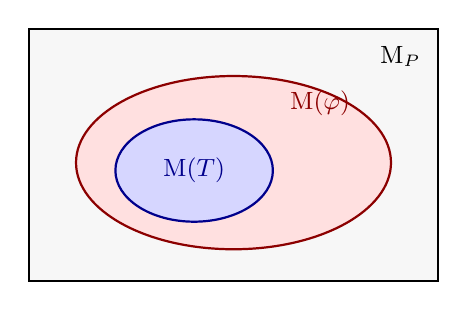
\begin{tikzpicture}[scale=1.0,font=\small]
  % univerzum vsech modelu
  \draw[thick,fill=black!3] (0,0) rectangle (5.2,3.2);
  \node[anchor=north east] at (5.1,3.1) {$\Mset_{\mathbb{P}}$};
  % M(fí)
  \draw[fill=red!12,draw=red!55!black,thick] (2.6,1.5) ellipse (2.0 and 1.1);
  \node[red!55!black] at (3.7,2.25) {$\Mset(\varphi)$};
  % M(T) uvnitr M(fí)
  \draw[fill=blue!16,draw=blue!55!black,thick] (2.1,1.4) ellipse (1.0 and 0.65);
  \node[blue!55!black] at (2.1,1.4) {$\Mset(T)$};
\end{tikzpicture}\obrpopis{Modely jako podmnožiny pole všech ohodnocení $\Mset_{\mathbb{P}}$. Zde $\Mset(T)\subseteq\Mset(\varphi)$, tj.\ $T\models\varphi$ ($\varphi$ je důsledek $T$). Kdyby $\Mset(\varphi)=\Mset_{\mathbb{P}}$, je $\varphi$ tautologie; kdyby $\Mset(\varphi)=\emptyset$, je sporný; jinak je nezávislý.}
\end{center}

\begin{definice}[Důsledky a vlastnosti teorie]
\emph{Důsledky} teorie jsou $\Csq(T)=\{\varphi:T\models\varphi\}$. Teorie $T$ je \emph{sporná}, nemá-li model (pak v~ní platí vše); \emph{bezesporná} (\emph{splnitelná}), má-li model; \emph{kompletní}, je-li bezesporná a~každý výrok je v~ní pravdivý, nebo lživý (žádný nezávislý) -- to ve~výrokové logice nastane \emph{právě tehdy, když má jediný model}. (V~predikátové logice se \uv{jediný model} zjemní na~\uv{jediný model až na~elementární ekvivalenci}, viz sekci~6.)
\end{definice}

\begin{poznamka}
\textbf{Věta o~dedukci} (konečná verze): pro konečnou teorii je $\varphi\in\Csq(\{\varphi_1,\dots,\varphi_n\})$ právě tehdy, když je $(\varphi_1\wedge\cdots\wedge\varphi_n)\to\varphi$ tautologie. Plyne přímo z~$\Mset(\varphi_1,\dots,\varphi_n)\subseteq\Mset(\varphi)\iff\models(\bigwedge\varphi_i)\to\varphi$. Z~existence DNF/CNF (sekce~1) navíc plyne \emph{funkční úplnost} systému $\{\neg,\wedge,\vee\}$: nad konečným $\mathbb{P}$ vyjádří každou booleovskou funkci, a~tedy každou množinu modelů, nějaký výrok.
\end{poznamka}

\begin{priklad}[Analýza teorie nad konečně mnoha prvovýroky]
\textbf{Zadání.}\par
Nad $\mathbb{P}=\{p,q,r\}$ uvažme $T=\{p\vee q\vee r,\ q\to r,\ \neg r\}$. (1)~Najděte všechny modely $T$. (2)~Rozhodněte, zda je $p$ pravdivý, lživý, či nezávislý v~$T$.

\smallskip
\textbf{Řešení.} Postupujeme od~nejselektivnějšího axiomu (zúžíme množinu kandidátů):
\begin{enumerate}[label=(\arabic*)]
  \item $\neg r$ vynutí $r=0$; zbývají $(p,q,r)\in\{(0,0,0),(0,1,0),(1,0,0),(1,1,0)\}$.\par
    $q\to r$ při $r=0$ vyžaduje $q=0$; zbývají $(0,0,0),(1,0,0)$.\par
    $p\vee q\vee r$ vyloučí $(0,0,0)$. Tedy $\boxed{\Mset(T)=\{(1,0,0)\}}$ -- jediný model.
  \item V~jediném modelu je $p=1$, takže $\Mset(T)\subseteq\Mset(p)$: $p$ je \textbf{pravdivý v~$T$} (a $T$ je dokonce kompletní, má jediný model).
\end{enumerate}
\end{priklad}

\begin{priklad}[Počítání nad konečným jazykem]
\textbf{Zadání.} Nad $\mathbb{P}$ s~$|\mathbb{P}|=n=3$ má bezesporná teorie $T$ právě $k=2$ modely. Kolik je (až na~ekvivalenci) výroků nezávislých v~$T$?

\smallskip
\textbf{Řešení.} Výrok až na~ekvivalenci určuje jeho množina modelů $M=\Mset(\varphi)\subseteq\Mset_{\mathbb{P}}$, kde $|\Mset_{\mathbb{P}}|=2^n=8$. Nezávislost v~$T$ znamená $\emptyset\neq M\cap\Mset(T)\neq\Mset(T)$: na~dvou modelech teorie máme $2^k-2=2$ \uv{netriviální} volby průniku, na~zbylých $2^n-k=6$ ohodnoceních volíme libovolně ($2^6$). Celkem $(2^k-2)\cdot2^{\,2^n-k}=2\cdot2^{6}=\boxed{128}$ výroků nezávislých v~$T$.
\end{priklad}

\subsection{Sémantika predikátové logiky}

V~predikátové logice nese význam \emph{struktura}: zvolí doménu a~realizuje (interpretuje) všechny symboly jazyka.

\begin{definice}[Struktura, model jazyka]
\emph{Struktura} (model jazyka $L$) je $\mathcal A=\langle A,\mathcal R^{\mathcal A},\mathcal F^{\mathcal A}\rangle$: neprázdná \emph{doména} $A$; pro každý $n$-ární relační symbol $R$ \emph{realizace} $R^{\mathcal A}\subseteq A^n$; pro každý $n$-ární funkční symbol $f$ realizace $f^{\mathcal A}\colon A^n\to A$ (pro konstantu $c$ je $c^{\mathcal A}\in A$).
\end{definice}

\begin{definice}[Hodnota termu, pravdivostní hodnota formule]
\emph{Ohodnocení proměnných} je $e\colon\mathrm{Var}\to A$; $e(x/a)$ změní hodnotu $x$ na~$a$. \emph{Hodnota termu} $t^{\mathcal A}[e]$: $x^{\mathcal A}[e]=e(x)$, $c^{\mathcal A}[e]=c^{\mathcal A}$, $f(t_1,\dots,t_n)^{\mathcal A}[e]=f^{\mathcal A}(t_1^{\mathcal A}[e],\dots,t_n^{\mathcal A}[e])$. \emph{Pravdivostní hodnota} $\mathrm{H}^{\mathcal A}(\varphi)[e]$ je dána indukcí:
\[
\mathrm{H}^{\mathcal A}\big(R(t_1,\dots,t_n)\big)[e]=1\iff(t_1^{\mathcal A}[e],\dots,t_n^{\mathcal A}[e])\in R^{\mathcal A},
\]
spojky přes pravdivostní tabulky a~pro kvantifikátory
\[
\mathrm{H}^{\mathcal A}\big((\forall x)\varphi\big)[e]=\min_{a\in A}\mathrm{H}^{\mathcal A}(\varphi)[e(x/a)],\qquad
\mathrm{H}^{\mathcal A}\big((\exists x)\varphi\big)[e]=\max_{a\in A}\mathrm{H}^{\mathcal A}(\varphi)[e(x/a)].
\]
\end{definice}

\begin{intuice}
Tarského definice: hodnotu formule počítáme \uv{zevnitř ven}. Kvantifikátor $\forall$ je \uv{konjunkce přes všechny prvky domény} (proto $\min$), $\exists$ je \uv{disjunkce přes prvky} (proto $\max$). Pozor na~záměnu symbolu a~jeho realizace: ve~struktuře $\langle\mathbb{N},\cdot,3\rangle$ jazyka $\langle+,1\rangle$ je $(x+1)$ vyhodnoceno jako $e(x)\cdot 3$.
\end{intuice}

\begin{definice}[Platnost, model teorie]
$\varphi$ \emph{platí v~$\mathcal A$ při~$e$}, $\mathcal A\models\varphi[e]$, je-li $\mathrm{H}^{\mathcal A}(\varphi)[e]=1$. $\varphi$ je \emph{pravdivá v~$\mathcal A$}, $\mathcal A\models\varphi$, platí-li při \emph{každém} $e$ (pro sentenci na~$e$ nezáleží); je \emph{lživá v~$\mathcal A$}, je-li $\mathcal A\models\neg\varphi$. \emph{Model teorie} $T$ je struktura, v~níž platí všechny axiomy ($\mathcal A\models T$); třída modelů je $\Mset_L(T)$. Sentence $\varphi$ je \emph{pravdivá / lživá / nezávislá v~$T$} přesně jako ve~výrokovém případě (přes $\Mset_L(T)$ a~$\Mset_L(\varphi)$); pravdivým sentencím říkáme \emph{důsledky}, $\Csq_L(T)$.
\end{definice}

\begin{poznamka}
\textbf{Lživá $\neq$ \uv{není pravdivá}}: u~formule s~volnou proměnnou může $\mathcal A\not\models\varphi$ i~$\mathcal A\not\models\neg\varphi$ (např.\ $\varphi=P(x)$, kde $P^{\mathcal A}$ je vlastní neprázdná podmnožina). Konkrétně pro $A=\{0,1\}$ a~$P^{\mathcal A}=\{0\}$: při $e(x)=0$ formule platí, při $e(x)=1$ neplatí, takže $P(x)$ není pravdivá (neplatí při každém $e$) ani lživá (neplatí $\neg P(x)$ při každém $e$). Pro \emph{sentence} už \uv{lživá} a~\uv{není pravdivá} splývají. \emph{Formule platí ve~struktuře právě tehdy, když v~ní platí její generální (univerzální) uzávěr.}
\end{poznamka}

\begin{poznamka}
\textbf{Jazyk s~rovností a~axiomy rovnosti.} Je-li $=$ v~jazyce, žádáme, aby se ve~všech uvažovaných strukturách interpretoval jako \emph{skutečná identita} na~doméně (relace \uv{být týž prvek}). V~dokazovacích systémech, kde je $=$ jen další relační symbol (tablo, rezoluce), tuto interpretaci vynutíme přidáním \emph{axiomů rovnosti}:
\begin{itemize}
  \item \emph{reflexivita:} $x=x$;
  \item \emph{slučitelnost s~funkcemi:} pro každý $n$-ární funkční symbol $f$
    \[ x_1=y_1\wedge\dots\wedge x_n=y_n\ \to\ f(x_1,\dots,x_n)=f(y_1,\dots,y_n); \]
  \item \emph{slučitelnost s~relacemi:} pro každý $n$-ární relační symbol $R$ (včetně samotného $=$)
    \[ x_1=y_1\wedge\dots\wedge x_n=y_n\ \to\ \big(R(x_1,\dots,x_n)\to R(y_1,\dots,y_n)\big). \]
\end{itemize}
Symetrii ($x=y\to y=x$) ani tranzitivitu ($x=y\wedge y=z\to x=z$) přidávat netřeba -- plynou z~reflexivity a~slučitelnosti aplikované na~$R$ rovné $=$. Tyto axiomy zaručí, že $={}^{\mathcal A}$ je \emph{kongruence}; faktorizací podle ní vznikne model, kde je $=$ skutečná identita.
\end{poznamka}

\begin{priklad}[Struktura jako model teorie]
\textbf{Zadání.} V~jazyce $\langle E\rangle$ s~rovností je \emph{teorie grafů} $T_{\mathrm{graf}}=\{\neg E(x,x),\ E(x,y)\to E(y,x)\}$ (ireflexivita, symetrie). Rozhodněte, zda je struktura $\mathcal G$ na~obrázku jejím modelem, a~zda je v~ní sentence $\psi=(\forall x)(\exists y)E(x,y)$ (\uv{každý vrchol má souseda}) pravdivá.

\smallskip
\textbf{Řešení.} Modely $T_{\mathrm{graf}}$ jsou přesně \emph{jednoduché grafy} ($E^{\mathcal A}$ je ireflexivní a~symetrická relace). Na~obrázku je $E^{\mathcal G}$ symetrická (hrany kreslíme neorientovaně) a~bez smyček, takže $\mathcal G\models T_{\mathrm{graf}}$. Sentence $\psi$ je pravdivá, právě když žádný vrchol není izolovaný; zde má každý vrchol aspoň jednu hranu, tedy $\mathcal G\models\psi$. (Naopak ve~struktuře s~izolovaným vrcholem by $\psi$ neplatila -- $\psi$ je v~$T_{\mathrm{graf}}$ \textbf{nezávislá}.)

\smallskip
\begin{center}
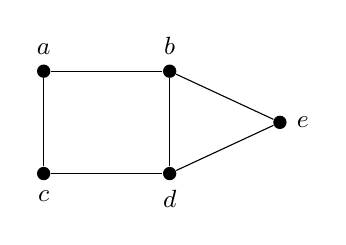
\begin{tikzpicture}[scale=1.0,font=\small,
  vert/.style={circle,fill=black,inner sep=1.7pt}]
  \node[vert,label=above:{$a$}] (a) at (0,1.3) {};
  \node[vert,label=above:{$b$}] (b) at (1.6,1.3) {};
  \node[vert,label=below:{$c$}] (c) at (0,0) {};
  \node[vert,label=below:{$d$}] (d) at (1.6,0) {};
  \node[vert,label=right:{$e$}] (e) at (3.0,0.65) {};
  \draw (a)--(b); \draw (a)--(c); \draw (b)--(d); \draw (c)--(d); \draw (b)--(e); \draw (d)--(e);
\end{tikzpicture}\obrpopis{Struktura $\mathcal G=\langle\{a,b,c,d,e\},E^{\mathcal G}\rangle$ jako model teorie grafů: $E^{\mathcal G}$ je symetrická (neorientované hrany) a~ireflexivní (bez smyček), tj.\ $\mathcal G\models\{\neg E(x,x),\,E(x,y)\to E(y,x)\}$. Žádný vrchol není izolovaný, proto $\mathcal G\models(\forall x)(\exists y)E(x,y)$.}
\end{center}
\end{priklad}

\begin{veta}[Platnost převedená na nesplnitelnost]
Je-li $T$ teorie a~$\varphi$ \emph{sentence} (téhož jazyka), pak
\[
T\models\varphi\quad\Longleftrightarrow\quad T\cup\{\neg\varphi\}\ \text{nemá model.}
\]
\end{veta}

\begin{proof}[Důkaz \textnormal{(nepovinný -- řetězec ekvivalencí)}]
$T\cup\{\neg\varphi\}$ nemá model $\iff$ $\neg\varphi$ neplatí v~žádném modelu $T$ $\iff$ (protože $\varphi$ je sentence) $\varphi$ platí v~každém modelu $T$ $\iff$ $T\models\varphi$.
\end{proof}

\begin{intuice}
Tato drobná věta je \emph{motor} dokazovacích metod: tablo i~rezoluce \uv{dokazují} $\varphi$ tak, že \emph{vyvrátí} (ukážou nesplnitelnost) $T\cup\{\neg\varphi\}$ -- důkaz sporem. Předpoklad \uv{$\varphi$ je sentence} je nutný (pro $\varphi=P(x)$, $T=\{P(c)\}$ věta selže).
\end{intuice}

% ============================================================
\section{Extenze teorií: síla, konzervativnost, skolemizace}\label{sec:extenze}

Často chceme jednu teorii \emph{rozšířit} -- přidat axiomy, nebo dokonce nové symboly -- a~ptát se, jak se změní její síla. Klíčové je, kdy rozšíření \uv{nic nového neřekne} o~původním jazyce (konzervativnost) a~jak teorii zjednodušit na~otevřenou (skolemizace), což je vstupní krok rezoluce.

\subsection{Extenze a porovnání síly teorií}

\begin{definice}[Extenze teorie]
Nechť $T$ je teorie v~jazyce $L$ a~$T'$ teorie v~jazyce $L'\supseteq L$.
\begin{itemize}
  \item $T'$ je \emph{extenze} $T$, pokud $\Csq_L(T)\subseteq\Csq_{L'}(T')$ (každý důsledek $T$ platí i~v~$T'$).
  \item Extenze je \emph{jednoduchá}, je-li $L'=L$ (beze změny jazyka).
  \item Extenze je \emph{konzervativní}, platí-li navíc $\Csq_L(T)=\Csq_{L'}(T')\cap\{L\text{-sentence}\}$ (v~původním jazyce $T'$ nedokáže nic nového).
  \item Teorie jsou \emph{ekvivalentní}, jsou-li navzájem svými extenzemi.
\end{itemize}
\end{definice}

\begin{intuice}
\uv{Více axiomů = méně modelů = silnější teorie.} Pro jednoduché extenze ($L'=L$) je $T'$ extenze $T$ právě tehdy, když $\Mset_L(T')\subseteq\Mset_L(T)$. \emph{Konzervativní} extenze smí používat nové symboly, ale o~starém jazyce říká přesně totéž co $T$ -- typicky jen zavádí pohodlnou \uv{zkratku}. To je přesně situace \emph{extenze o~definice}.
\end{intuice}

\begin{veta}[Sémantické kritérium extenze]
Nechť $L\subseteq L'$, $T$ v~$L$, $T'$ v~$L'$. Pak:
\begin{enumerate}[label=\emph{(\roman*)}]
  \item $T'$ je extenze $T$ právě tehdy, když $L$-redukt každého modelu $T'$ je modelem $T$;
  \item je-li $T'$ extenze $T$ a~lze-li \emph{každý} model $T$ expandovat (dointerpretováním nových symbolů) na~model $T'$, je $T'$ \emph{konzervativní} extenze $T$.
\end{enumerate}
\end{veta}

\begin{poznamka}
\textbf{Věta o~konstantách} (podpůrná): rozšíříme-li $L$ o~nové konstanty $c_1,\dots,c_n$ a~$T$ ponecháme, pak pro formuli $\varphi(x_1,\dots,x_n)$ platí $T\models\varphi$ právě tehdy, když $T\models\varphi(x_1/c_1,\dots,x_n/c_n)$ v~rozšířeném jazyce. \uv{Volná proměnná} a~\uv{nová konstanta nesvázaná axiomy} jsou tedy zaměnitelné; tohoto triku využijí \uv{svědci} v~tablo metodě (sekce~\ref{sec:dokaz}).
\end{poznamka}

\subsection{Extenze o definice}

Nejdůležitější konzervativní extenze zavádí \emph{definovaný symbol} pohodlnou zkratkou.

\begin{definice}[Extenze o definici relačního a funkčního symbolu]
Nechť $T$ je teorie v~$L$.
\begin{itemize}
  \item \emph{Definice relačního symbolu:} pro formuli $\psi(x_1,\dots,x_n)$ a~nový $n$-ární relační symbol $R$ je $T'=T\cup\{R(x_1,\dots,x_n)\leftrightarrow\psi(x_1,\dots,x_n)\}$.
  \item \emph{Definice funkčního symbolu:} pro $\psi(x_1,\dots,x_n,y)$ a~nový $n$-ární funkční symbol $f$, \emph{pokud v~$T$ platí} axiom existence $(\exists y)\psi$ a~jednoznačnosti $\psi(\bar x,y)\wedge\psi(\bar x,z)\to y=z$, je $T'=T\cup\{f(x_1,\dots,x_n)=y\leftrightarrow\psi(x_1,\dots,x_n,y)\}$.
\end{itemize}
\end{definice}

\begin{dusledek}[Konzervativnost]
Extenze o~definice je \emph{konzervativní} (každý model $T$ se rozšíří na~model $T'$, navíc \emph{jednoznačně}). Pro každou $L'$-formuli $\varphi'$ existuje $L$-formule $\varphi$ s~$T'\models\varphi'\leftrightarrow\varphi$ -- definovaný symbol lze vždy \uv{rozvést} zpět.
\end{dusledek}

\begin{intuice}
Ekvivalence $R(\bar x)\leftrightarrow\psi(\bar x)$ \emph{jednoznačně} dourčí interpretaci nového $R$ z~modelu $T$, takže nepřibudou ani neubudou modely (až na~nový symbol). U~funkce je navíc třeba, aby $\psi$ definovala \emph{totální a~jednoznačnou} relaci -- proto axiomy existence a~jednoznačnosti (např.\ $\min$ lze definovat až nad \emph{lineárním} uspořádáním; $\tfrac12$ až nad tělesem charakteristiky $\neq 2$).
\end{intuice}

\begin{priklad}[Rozvedení definovaného symbolu]
\textbf{Zadání.} Nad teorií uspořádaných grup $T$ jazyka $\langle+,0,\le\rangle$ (s~rovností) zaveďme \emph{inverzní prvek} $-$ definicí $-x=y\leftrightarrow x+y=0$ a~ostré uspořádání $<$ pomocí $\le$ definicí $x<y\leftrightarrow(x\le y\wedge\neg\,x=y)$. Rozveďte formuli $-x<y$ na~formuli původního jazyka.

\smallskip
\textbf{Řešení.} Definovaný term $-x$ nahradíme novou proměnnou $z$ vázanou existenčním kvantifikátorem (a~dodáme definující podmínku $x+z=0$); definovaný predikát $<$ rozepíšeme:
\[
-x<y\ \equiv_{T'}\ (\exists z)\big(\underbrace{(z\le y\wedge\neg\,z=y)}_{z<y}\ \wedge\ \underbrace{x+z=0}_{z=-x}\big).
\]
Výsledná formule je v~jazyce $\langle+,0,\le\rangle$ a~je $T'$-ekvivalentní s~$-x<y$.
\end{priklad}

\subsection{Skolemizace}

Skolemizace odstraní existenční kvantifikátory zavedením nových funkčních symbolů (\uv{svědků jako funkcí}) a~převede teorii na~\emph{otevřenou} -- za~cenu, že nová teorie je s~původní \emph{ekvisplnitelná}, ne nutně ekvivalentní. To stačí pro důkaz sporem (rezoluci).

\begin{definice}[Ekvisplnitelnost]
Teorie $T$ a~$T'$ (i~v~různých jazycích) jsou \emph{ekvisplnitelné}, pokud platí: $T$ má model právě tehdy, když $T'$ má model.
\end{definice}

\begin{definice}[Skolemova varianta]
Nechť $\varphi=(\forall x_1)\cdots(\forall x_m)(\exists y)\psi$ je sentence v~PNF, kde před $(\exists y)$ stojí právě univerzální kvantifikátory $(\forall x_1),\dots,(\forall x_m)$. Zavedeme nový $m$-ární funkční symbol $f$ a~nahradíme $\varphi$ za $(\forall x_1)\cdots(\forall x_m)\,\psi\big(y/f(x_1,\dots,x_m)\big)$. Opakováním přes všechny existenční kvantifikátory (vždy zleva) vznikne \emph{Skolemova varianta} $\varphi^S$; postupu říkáme \emph{skolemizace}. Arita každého $f$ je počet univerzálních kvantifikátorů nalevo od~rušeného $\exists$ -- nestojí-li nalevo žádný, je $f$ \emph{konstanta}.
\end{definice}

\begin{veta}[Skolemova věta]
Každá teorie má \emph{otevřenou konzervativní extenzi}. Speciálně každá sentence $\varphi$ je se~svou Skolemovou variantou $\varphi^S$ \emph{ekvisplnitelná}.
\end{veta}

\begin{intuice}
\uv{Existuje $y$} pro každou volbu $x_1,\dots,x_m$ znamená, že $y$ je \emph{funkcí} těchto $x_i$; tu funkci pojmenujeme novým $f$ a~$y$ jí nahradíme (volba svědka = axiom výběru). Skolemova varianta $\varphi^S$ \emph{není} ekvivalentní $\varphi$ (mluví o~bohatším jazyce), ale je s~ní ekvisplnitelná, což pro hledání sporu stačí. Postup: \emph{PNF $\to$ generální uzávěr (sentence!) $\to$ skolemizace $\to$ vypuštění $\forall$ $\to$ CNF}. Pozor: skolemizovat se musí ze~\emph{sentence} -- pro $(\exists y)E(x,y)$ není $E(x,c)$ Skolemova varianta (napřed generální uzávěr $(\forall x)(\exists y)E(x,y)$, pak $E(x,f(x))$).
\end{intuice}

\begin{priklad}[Skolemizace]
\textbf{Zadání.} Skolemizujte sentence (a)~$(\forall x)(\exists y)(\forall z)(\exists w)\,P(x,y,z,w)$ a~(b)~$(\exists y)(\forall x)\,Q(x,y)$.

\smallskip
\textbf{Řešení.}
\begin{enumerate}[label=(\alph*)]
  \item Před $(\exists y)$ stojí $(\forall x)$ $\Rightarrow$ $y\mapsto f(x)$ (unární $f$); před $(\exists w)$ stojí $(\forall x),(\forall z)$ $\Rightarrow$ $w\mapsto g(x,z)$ (binární $g$). Po~vypuštění $\forall$:
    \[
    \boxed{P\big(x,f(x),z,g(x,z)\big)}\quad(\text{otevřené jádro Skolemovy varianty}).
    \]
  \item Před $(\exists y)$ nestojí žádný $\forall$ $\Rightarrow$ $y\mapsto c$ (konstanta). Výsledek: $\boxed{Q(x,c)}$.
\end{enumerate}
Obě otevřené formule jsou s~původními sentencemi ekvisplnitelné a~lze je rovnou převést do~CNF (množiny klauzulí) pro rezoluci.
\end{priklad}

% ============================================================
\section{Dokazatelnost: tablo metoda, rezoluce, Hilbert}\label{sec:dokaz}

Dokazovací systém formalizuje \uv{dokazování} jako syntaktickou proceduru: \emph{důkaz} je konečný objekt, který lze algoritmicky ověřit. Píšeme $T\vdash\varphi$ (\uv{$\varphi$ je dokazatelná z~$T$}). Žádáme \emph{korektnost} ($T\vdash\varphi\Rightarrow T\models\varphi$ -- co dokážeme, platí) a~ideálně \emph{úplnost} ($T\models\varphi\Rightarrow T\vdash\varphi$ -- co platí, dokážeme). Tablo i~rezoluce dokazují \emph{sporem}: vyvrátí $T\cup\{\neg\varphi\}$.

\subsection{Tablo metoda ve výrokové logice}

\begin{definice}[Tablo, položka, tablo důkaz]
\emph{Položka} je $T\psi$ nebo $F\psi$ (\uv{$\psi$ v~hledaném modelu platí / neplatí}). \emph{Tablo} z~teorie $T$ je strom označkovaný položkami, který vzniká z~kořene \emph{redukcemi} (připojením \emph{atomického tabla} pro položku na~větvi dle tabulky níže) a~připojením $T\alpha$ pro libovolný axiom $\alpha\in T$. Větev je \emph{sporná} (značka~\closed), obsahuje-li $T\psi$ i~$F\psi$; \emph{dokončená}, je-li sporná nebo má všechny položky zredukované a~obsahuje všechny axiomy. \emph{Tablo důkaz $\varphi$ z~$T$} je \emph{sporné} tablo s~$F\varphi$ v~kořeni (tehdy $T\vdash\varphi$); \emph{zamítnutí} je sporné tablo s~$T\varphi$ v~kořeni.
\end{definice}

\begin{center}
\renewcommand{\arraystretch}{1.15}
\begin{tabular}{ll@{\qquad}ll}
\toprule
položka & rozvoj & položka & rozvoj\\
\midrule
$T\,\neg\varphi$ & $F\varphi$ & $F\,\neg\varphi$ & $T\varphi$\\
$T(\varphi\wedge\psi)$ & $T\varphi,\,T\psi$ & $F(\varphi\wedge\psi)$ & $F\varphi\ \mid\ F\psi$\\
$T(\varphi\vee\psi)$ & $T\varphi\ \mid\ T\psi$ & $F(\varphi\vee\psi)$ & $F\varphi,\,F\psi$\\
$T(\varphi\to\psi)$ & $F\varphi\ \mid\ T\psi$ & $F(\varphi\to\psi)$ & $T\varphi,\,F\psi$\\
$T(\varphi\leftrightarrow\psi)$ & $T\varphi,T\psi\ \mid\ F\varphi,F\psi$ & $F(\varphi\leftrightarrow\psi)$ & $T\varphi,F\psi\ \mid\ F\varphi,T\psi$\\
\bottomrule
\end{tabular}\\[1mm]
{\small Atomická tabla. Čárka \uv{$,$} = položky pod sebou na~téže větvi; svislítko \uv{$\mid$} = rozvětvení. (Pravidla čtou \uv{jak může položka nastat}: $F(\varphi\to\psi)$ jen tak, že platí $\varphi$ a~neplatí $\psi$.)}
\end{center}

\begin{intuice}
Tablo \emph{hledá protipříklad}: do~kořene dáme $F\varphi$ (\uv{kéž $\varphi$ neplatí}) a~rozvíjíme důsledky. \emph{Sporná} větev (\closed) znamená, že protipříklad na~ní neexistuje; \emph{každá} větev sporná $\Rightarrow$ protipříklad neexistuje vůbec $\Rightarrow$ $\varphi$ platí. Naopak \emph{dokončená bezesporná} větev dává \emph{protipříklad}: \uv{kanonický model} $v(p)=1$ právě když je na~větvi $Tp$.
\end{intuice}

\begin{center}
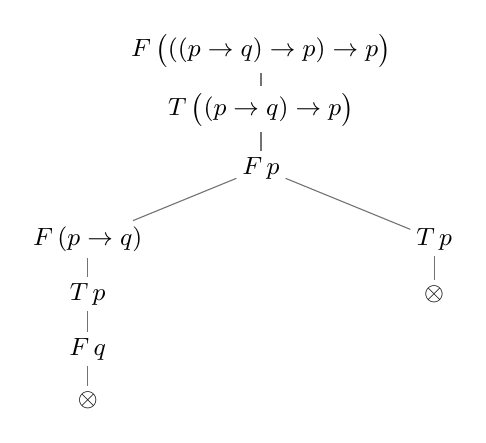
\begin{tikzpicture}[font=\small,every node/.style={inner sep=2pt},lvl/.style={draw=black!55}]
  \node (n1) at (0,0) {$F\,\big(((p\to q)\to p)\to p\big)$};
  \node (n2) at (0,-0.75) {$T\,\big((p\to q)\to p\big)$};
  \node (n3) at (0,-1.5) {$F\,p$};
  \node (l1) at (-2.2,-2.4) {$F\,(p\to q)$};
  \node (r1) at (2.2,-2.4) {$T\,p$};
  \node (l2) at (-2.2,-3.1) {$T\,p$};
  \node (l3) at (-2.2,-3.8) {$F\,q$};
  \node (lx) at (-2.2,-4.45) {\closed};
  \node (rx) at (2.2,-3.1) {\closed};
  \draw[black!55] (n1)--(n2)--(n3);
  \draw[black!55] (n3)--(l1); \draw[black!55] (n3)--(r1);
  \draw[black!55] (l1)--(l2)--(l3)--(lx); \draw[black!55] (r1)--(rx);
\end{tikzpicture}\obrpopis{Tablo důkaz Peirceova zákona $\big((p\to q)\to p\big)\to p$. Kořen $F\varphi$; po~redukci $F{\to}$ máme $T((p{\to}q){\to}p)$ a~$Fp$, redukce $T{\to}$ větví na~$F(p{\to}q)\mid Tp$. Pravá větev: $Tp$ proti $Fp$ \closed. Levá: $F(p{\to}q)$ dá $Tp,Fq$, opět $Tp$ proti $Fp$ \closed. Obě větve sporné $\Rightarrow$ $\vdash\varphi$ (tautologie).}
\end{center}

\begin{priklad}[Tablo: důkaz vs.\ protipříklad]
\textbf{Zadání.}\par
(1)~Dokažte tablo metodou, že $\{\neg q,\ p\vee q\}\models p$. (2)~Tablo metodou rozhodněte, zda je $(\neg q\vee p)\to p$ tautologie.

\smallskip
\textbf{Řešení.}
\begin{enumerate}[label=(\arabic*)]
  \item Kořen $Fp$; připojíme axiomy $T\neg q$ a~$T(p\vee q)$. Redukce $T\neg q\rightsquigarrow Fq$. Redukce $T(p\vee q)$ \emph{větví} na~$Tp\mid Tq$: levá $Tp$ proti $Fp$ \closed, pravá $Tq$ proti $Fq$ \closed. Obě sporné $\Rightarrow$ $\{\neg q,p\vee q\}\vdash p$, tedy (korektnost) i~$\models p$.
  \item Kořen $F\big((\neg q\vee p)\to p\big)$; redukce $F{\to}$ dá $T(\neg q\vee p)$ a~$Fp$. Redukce $T(\neg q\vee p)$ větví na~$T\neg q\mid Tp$: pravá $Tp$ proti $Fp$ \closed; levá $T\neg q\rightsquigarrow Fq$ je \textbf{dokončená a~bezesporná} ($Fp,Fq$). Kanonický model $v=(p{=}0,q{=}0)$: $(\neg q\vee p)=1$, ale $p=0$, takže $1\to 0=0$ -- \textbf{protipříklad}. Formule \emph{není} tautologie.
\end{enumerate}

\smallskip
\begin{minipage}[t]{0.46\linewidth}\centering
{\small (1) sporné tablo $=$ důkaz}\\[1mm]
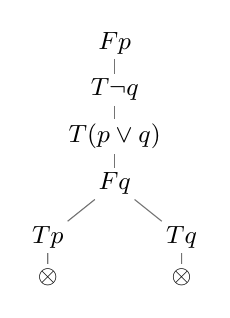
\begin{tikzpicture}[scale=0.85,font=\small,every node/.style={inner sep=1.6pt}]
  \node (a) at (0,0) {$Fp$};
  \node (b) at (0,-0.7) {$T\neg q$};
  \node (c) at (0,-1.4) {$T(p\vee q)$};
  \node (d) at (0,-2.1) {$Fq$};
  \node (l) at (-1,-2.9) {$Tp$};
  \node (r) at (1,-2.9) {$Tq$};
  \node (lx) at (-1,-3.5) {\closed};
  \node (rx) at (1,-3.5) {\closed};
  \draw[black!55] (a)--(b)--(c)--(d); \draw[black!55] (d)--(l); \draw[black!55] (d)--(r);
  \draw[black!55] (l)--(lx); \draw[black!55] (r)--(rx);
\end{tikzpicture}\\[0.5mm]
{\footnotesize Obě větve sporné: $\{\neg q,\,p\vee q\}\vdash p$.}
\end{minipage}\hfill
\begin{minipage}[t]{0.46\linewidth}\centering
{\small (2) otevřená větev $=$ protimodel}\\[1mm]
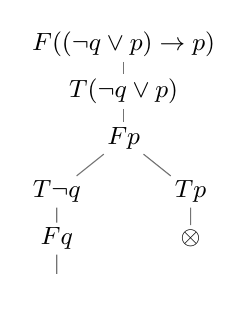
\begin{tikzpicture}[scale=0.85,font=\small,every node/.style={inner sep=1.6pt}]
  \node (a) at (0,0) {$F((\neg q\vee p)\to p)$};
  \node (b) at (0,-0.7) {$T(\neg q\vee p)$};
  \node (c) at (0,-1.4) {$Fp$};
  \node (l) at (-1,-2.2) {$T\neg q$};
  \node (r) at (1,-2.2) {$Tp$};
  \node (lq) at (-1,-2.9) {$Fq$};
  \node (lo) at (-1,-3.5) {\open};
  \node (rx) at (1,-2.9) {\closed};
  \draw[black!55] (a)--(b)--(c); \draw[black!55] (c)--(l); \draw[black!55] (c)--(r);
  \draw[black!55] (l)--(lq)--(lo); \draw[black!55] (r)--(rx);
\end{tikzpicture}\\[0.5mm]
{\footnotesize Větev $\{Fp,Fq\}$ bezesporná $\Rightarrow$ protimodel $(0,0)$.}
\end{minipage}
\end{priklad}

\subsection{Tablo metoda v predikátové logice}

V~PL pracují položky se~\emph{sentencemi} (formuli i~axiomy nahradíme generálními uzávěry). Spojkové rozvoje jsou stejné, přibývají \emph{kvantifikátorová} pravidla dvojího druhu:

\begin{center}
\renewcommand{\arraystretch}{1.2}
\begin{tabular}{ll}
\toprule
\textbf{typ \uv{všichni}} (libovolný term $t$) & \textbf{typ \uv{svědek}} (nový konstantní symbol $c$)\\
\midrule
$T(\forall x)\varphi(x)\ \rightsquigarrow\ T\varphi(x/t)$ & $T(\exists x)\varphi(x)\ \rightsquigarrow\ T\varphi(x/c)$\\
$F(\exists x)\varphi(x)\ \rightsquigarrow\ F\varphi(x/t)$ & $F(\forall x)\varphi(x)\ \rightsquigarrow\ F\varphi(x/c)$\\
\bottomrule
\end{tabular}
\end{center}

\begin{intuice}
\uv{Svědek} ($T\exists$, $F\forall$): existenci dosvědčí \emph{nový} konstantní symbol $c$ -- pojmenuje onen prvek (formálně věta o~konstantách). \uv{Všichni} ($T\forall$, $F\exists$): smíme dosadit \emph{libovolný} term, a~aby byla větev dokončená, musíme postupně dosadit \emph{všechny} termy (proto tato položka zůstává \uv{nehotová} a~může generovat nekonečnou větev). V~jazyce s~rovností přidáme \emph{axiomy rovnosti} (reflexivita a~slučitelnost $=$ s~funkcemi i~relacemi), které vynutí, že $=$ se chová jako identita.
\end{intuice}

\begin{center}
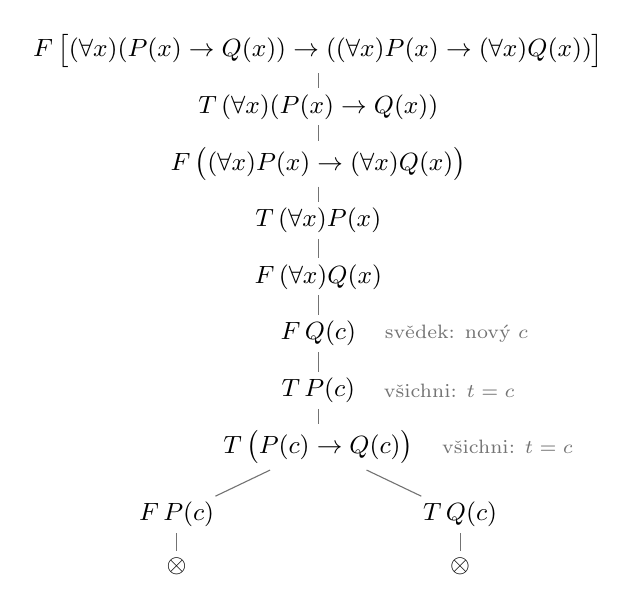
\begin{tikzpicture}[font=\small,every node/.style={inner sep=2pt}]
  \node (n1) at (0,0) {$F\,\big[(\forall x)(P(x)\to Q(x))\to((\forall x)P(x)\to(\forall x)Q(x))\big]$};
  \node (n2) at (0,-0.72) {$T\,(\forall x)(P(x)\to Q(x))$};
  \node (n3) at (0,-1.44) {$F\,\big((\forall x)P(x)\to(\forall x)Q(x)\big)$};
  \node (n4) at (0,-2.16) {$T\,(\forall x)P(x)$};
  \node (n5) at (0,-2.88) {$F\,(\forall x)Q(x)$};
  \node (n6) at (0,-3.60) {$F\,Q(c)$};
  \node (n7) at (0,-4.32) {$T\,P(c)$};
  \node (n8) at (0,-5.04) {$T\,\big(P(c)\to Q(c)\big)$};
  \node (l)  at (-1.8,-5.9) {$F\,P(c)$};
  \node (r)  at (1.8,-5.9) {$T\,Q(c)$};
  \node (lx) at (-1.8,-6.55) {\closed};
  \node (rx) at (1.8,-6.55) {\closed};
  \draw[black!55] (n1)--(n2)--(n3)--(n4)--(n5)--(n6)--(n7)--(n8);
  \draw[black!55] (n8)--(l); \draw[black!55] (n8)--(r);
  \draw[black!55] (l)--(lx); \draw[black!55] (r)--(rx);
  \node[anchor=west,font=\scriptsize,black!55] at ([xshift=6pt]n6.east) {svědek: nový $c$};
  \node[anchor=west,font=\scriptsize,black!55] at ([xshift=6pt]n7.east) {všichni: $t=c$};
  \node[anchor=west,font=\scriptsize,black!55] at ([xshift=6pt]n8.east) {všichni: $t=c$};
\end{tikzpicture}\obrpopis{Tablo důkaz $(\forall x)(P(x)\to Q(x))\to\big((\forall x)P(x)\to(\forall x)Q(x)\big)$. Z~$F\forall$ vznikne svědek $FQ(c)$; položky \uv{všichni} $T(\forall x)P$ a~$T(\forall x)(P\to Q)$ dosadíme týž $c$. Redukce $T(P(c){\to}Q(c))$ větví: $FP(c)$ proti $TP(c)$ \closed, $TQ(c)$ proti $FQ(c)$ \closed. Obě větve sporné $\Rightarrow$ formule je dokazatelná.}
\end{center}

\subsection{Rezoluční metoda ve výrokové logice}

Rezoluce pracuje s~CNF v~\emph{množinové reprezentaci}: \emph{klauzule} je množina literálů, \emph{formule} je množina klauzulí, prázdná klauzule $\eclause$ je nesplnitelná. Má jediné pravidlo a~dokazuje sporem (zamítnutím).

\begin{definice}[Rezoluční pravidlo, zamítnutí]
Mají-li klauzule $C_1$ literál $\ell$ a~$C_2$ opačný literál $\overline{\ell}$, je jejich \emph{rezolventa} (přes $\ell$)
\[
C=(C_1\setminus\{\ell\})\cup(C_2\setminus\{\overline{\ell}\}).
\]
\emph{Rezoluční důkaz} klauzule $C$ z~formule $S$ je posloupnost klauzulí končící $C$, kde každá je z~$S$ nebo rezolventou dvou předchozích. \emph{Zamítnutí} $S$ je rezoluční důkaz $\eclause$; pak je $S$ nesplnitelná.
\end{definice}

\begin{intuice}
Rezoluce je pravidlo řezu: z~$\ell\vee A$ a~$\overline\ell\vee B$ plyne $A\vee B$ (ať je $\ell$ pravdivý či ne, jedna z~klauzulí to \uv{nepokryje}, takže platí zbytek). Odvození $\eclause$ znamená, že požadavky jsou neslučitelné. Pozor: \emph{nelze} řezat přes dvě dvojice naráz -- $\{p,q\},\{\neg p,\neg q\}$ dají jen $\{q,\neg q\}$ či $\{p,\neg p\}$ (tautologie), nikoli $\eclause$ (a~jsou splnitelné).
\end{intuice}

\begin{center}
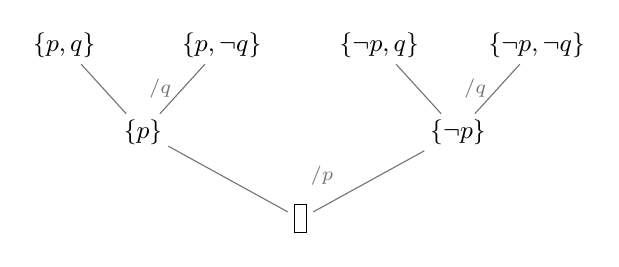
\begin{tikzpicture}[font=\small,every node/.style={inner sep=2pt},
  cl/.style={}]
  \node (a) at (-3,0) {$\{p,q\}$};
  \node (b) at (-1,0) {$\{p,\neg q\}$};
  \node (c) at (1,0) {$\{\neg p,q\}$};
  \node (d) at (3,0) {$\{\neg p,\neg q\}$};
  \node (p) at (-2,-1.1) {$\{p\}$};
  \node (np) at (2,-1.1) {$\{\neg p\}$};
  \node (box) at (0,-2.2) {$\eclause$};
  \draw[black!55] (a)--(p); \draw[black!55] (b)--(p);
  \draw[black!55] (c)--(np); \draw[black!55] (d)--(np);
  \draw[black!55] (p)--(box); \draw[black!55] (np)--(box);
  \node[anchor=west,black!55] at (-2.0,-0.55) {\scriptsize $/q$};
  \node[anchor=west,black!55] at (2.0,-0.55) {\scriptsize $/q$};
  \node[anchor=west,black!55] at (0.05,-1.65) {\scriptsize $/p$};
\end{tikzpicture}\obrpopis{Rezoluční strom: zamítnutí nesplnitelné $S=\{\{p,q\},\{p,\neg q\},\{\neg p,q\},\{\neg p,\neg q\}\}$. Řez přes $q$ dá $\{p\}$ a~$\{\neg p\}$, řez přes $p$ dá $\eclause$. Listy jsou klauzule z~$S$, kořen je $\eclause$.}
\end{center}

\begin{priklad}[Rezoluční důkaz v teorii]
\textbf{Zadání.}\par
Rezolucí dokažte, že z~$T=\{\neg p\to\neg q,\ \neg q\to\neg r,\ (r\to p)\to s\}$ plyne $s$.

\smallskip
\textbf{Řešení.} Podle věty \uv{platnost = nesplnitelnost} stačí zamítnout $T\cup\{\neg s\}$. Převod do~CNF (kritický je třetí axiom: $(r\to p)\to s\sim(r\vee s)\wedge(\neg p\vee s)$):
\[
S=\big\{\{p,\neg q\},\ \{q,\neg r\},\ \{r,s\},\ \{\neg p,s\},\ \{\neg s\}\big\}.
\]
Zamítnutí (každý krok = řez přes vyznačený literál):
\[
\{\neg s\},\{r,s\}\xrightarrow{/s}\{r\};\quad
\{r\},\{q,\neg r\}\xrightarrow{/r}\{q\};\quad
\{q\},\{p,\neg q\}\xrightarrow{/q}\{p\};
\]
\[
\{\neg s\},\{\neg p,s\}\xrightarrow{/s}\{\neg p\};\quad
\{p\},\{\neg p\}\xrightarrow{/p}\boxed{\eclause.}
\]
Tedy $T\cup\{\neg s\}$ je nesplnitelná, a~proto $T\models s$.

\smallskip
\begin{center}
\begin{tikzpicture}[font=\small,every node/.style={inner sep=2pt}]
  \node (rs)  at (-3.3, 0)    {$\{r,s\}$};
  \node (ns1) at (-1.9, 0)    {$\{\neg s\}$};
  \node (qnr) at (-0.4,-1.1)  {$\{q,\neg r\}$};
  \node (pnq) at ( 0.7,-2.2)  {$\{p,\neg q\}$};
  \node (ns2) at ( 2.0,-2.2)  {$\{\neg s\}$};
  \node (nps) at ( 3.6,-2.2)  {$\{\neg p,s\}$};
  \node (r)   at (-2.6,-1.1)  {$\{r\}$};
  \node (q)   at (-1.5,-2.2)  {$\{q\}$};
  \node (p)   at (-0.4,-3.3)  {$\{p\}$};
  \node (np)  at ( 2.8,-3.3)  {$\{\neg p\}$};
  \node (box) at ( 1.2,-4.4)  {$\eclause$};
  \draw[black!55] (rs)--(r);  \draw[black!55] (ns1)--(r);
  \draw[black!55] (r)--(q);   \draw[black!55] (qnr)--(q);
  \draw[black!55] (q)--(p);   \draw[black!55] (pnq)--(p);
  \draw[black!55] (ns2)--(np);\draw[black!55] (nps)--(np);
  \draw[black!55] (p)--(box); \draw[black!55] (np)--(box);
  \node[anchor=west,black!55,fill=white,inner sep=1pt] at (-2.55,-0.62) {\scriptsize $/s$};
  \node[anchor=west,black!55,fill=white,inner sep=1pt] at (-1.45,-1.72) {\scriptsize $/r$};
  \node[anchor=west,black!55,fill=white,inner sep=1pt] at (-0.35,-2.82) {\scriptsize $/q$};
  \node[anchor=west,black!55,fill=white,inner sep=1pt] at ( 2.85,-2.82) {\scriptsize $/s$};
  \node[anchor=west,black!55,fill=white,inner sep=1pt] at ( 1.25,-3.92) {\scriptsize $/p$};
\end{tikzpicture}\obrpopis{Rezoluční strom zamítnutí $S=T\cup\{\neg s\}$. Levá větev řezy přes $s,r,q$ vyrobí $\{p\}$, vpravo z~$\{\neg s\}$ a~$\{\neg p,s\}$ vznikne $\{\neg p\}$; řez přes $p$ dá $\eclause$. Klauzule $\{\neg s\}$ vstupuje do~dvou řezů, proto je listem dvakrát. Listy jsou klauzule z~$S$, kořen je~$\eclause$.}
\end{center}
\end{priklad}

\subsection{Rezoluce v predikátové logice}

Po~skolemizaci (sekce~\ref{sec:extenze}) je teorie množinou klauzulí s~termy a~proměnnými. Rezoluce přibírá \emph{unifikaci}: před řezem ztotožníme literály substitucí.

\begin{definice}[Unifikace, rezoluční pravidlo s unifikací]
\emph{Substituce} $\sigma$ je nejobecnější \emph{unifikace} (\emph{mgu}) množiny výrazů $\{E_1,\dots,E_k\}$, je-li $E_1\sigma=\dots=E_k\sigma$ a~každá jiná unifikace přes ni \uv{vznikne}. \emph{Rezoluční pravidlo}: klauzule $C_1,C_2$ s~disjunktními proměnnými, $C_1=C_1'\cup\{A_1,\dots,A_n\}$, $C_2=C_2'\cup\{\neg B_1,\dots,\neg B_m\}$; je-li $\sigma$ mgu množiny $\{A_1,\dots,A_n,B_1,\dots,B_m\}$, je rezolventou $C=C_1'\sigma\cup C_2'\sigma$.
\end{definice}

\begin{intuice}
\emph{Unifikátor} množiny výrazů je substituce, která je syntakticky \emph{ztotožní} ($E_1\sigma=\dots=E_k\sigma$). \emph{Nejobecnější} z~nich (mgu) je \uv{nejméně zavazující}: sváže jen nezbytné a~každý jiný unifikátor $\theta$ z~něj vznikne dodatečným dosazením, $\theta=\sigma\lambda$. Např.\ $P(x)$ a~$P(y)$ má mgu $\sigma=\{x/y\}$ (výsledek $P(y)$); také $\theta=\{x/a,\,y/a\}$ je unifikuje, ale \emph{konkrétněji} ($\theta=\sigma\lambda$ s~$\lambda=\{y/a\}$) -- zbytečně se upnul na~$a$. V~rezoluci proto bereme \emph{vždy mgu}: s~konkrétnější unifikací bychom ztratili obecnost rezolventy a~rezoluce by nebyla úplná (mgu je jednoznačný až na~přejmenování proměnných).\par
Klauzule mají \emph{lokální} proměnné (implicitně univerzálně kvantované), proto je před řezem přejmenujeme na~disjunktní a~pak \emph{unifikujeme} řezané literály nejobecnějším způsobem (mgu). \emph{Mgu hledáme zleva}: porovnáváme termy a~vynucujeme potřebné rovnosti. Např.\ $P(f(x),y)$ a~$P(f(a),w)$ unifikuje $\sigma=\{x/a,\ y/w\}$; naopak $x$ a~$f(x)$ unifikovat \emph{nelze}, protože $x$ se vyskytuje uvnitř $f(x)$ (tzv.\ \emph{occurs-check}). Na~rozdíl od~výrokové logiky je dovoleno řezat přes \emph{více} literálů naráz: po~unifikaci se totiž dva literály téže klauzule mohou ztotožnit (\uv{faktorizace}), např.\ $\{P(x),P(y)\}$ se přes $\{x/y\}$ slije na~$\{P(y)\}$. Korektnost a~úplnost zůstávají (úplnost se \uv{zvedne} z~výrokové přes Herbrandovu větu).
\end{intuice}

\begin{priklad}[Rezoluce v PL: holičův paradox]
\textbf{Zadání.}\par
\uv{Každý holič holí právě ty, kdo neholí sami sebe.} Dokažte rezolucí, že \emph{žádný holič neexistuje}. Jazyk $\langle B,S\rangle$ ($B(x)$ -- \uv{$x$ je holič}, $S(x,y)$ -- \uv{$x$ holí $y$}).

\smallskip
\textbf{Řešení.}

\emph{Formalizace.}\\
\uv{Holič holí právě ty, kdo neholí sami sebe} dává ekvivalenci $S(x,y)\leftrightarrow\neg S(y,y)$ platnou pro každého $y$, jakmile je $x$ holič:
\[
T=\big\{(\forall x)\big(B(x)\to(\forall y)(S(x,y)\leftrightarrow\neg S(y,y))\big)\big\}.
\]
Dokazované tvrzení je $\psi=\neg(\exists x)B(x)$ (\uv{neexistuje holič}); podle \uv{platnost = nesplnitelnost} zamítáme $T\cup\{\neg\psi\}$, kde $\neg\psi=(\exists x)B(x)$.

\smallskip
\emph{Skolemizace a~CNF.}\\
Jediný existenční kvantifikátor je v~negovaném cíli.
\begin{itemize}
  \item \emph{Negovaný cíl} $(\exists x)B(x)$: před $\exists x$ nestojí žádný $\forall$, svědek je tedy \emph{konstanta} $c$ -- vznikne $B(c)$ (klauzule $C_3$).
  \item \emph{Premisa}: po~rozepsání $\leftrightarrow$ a~zatažení $B(x)$ pod $\forall y$ je \emph{čistě univerzální}
    \[
    (\forall x)(\forall y)\Big(B(x)\to\big[(S(x,y)\to\neg S(y,y))\wedge(\neg S(y,y)\to S(x,y))\big]\Big),
    \]
    takže \emph{neobsahuje žádný $\exists$ a~skolemizovat není co} (žádné Skolemovy funkce).
\end{itemize}
Vypuštěním $\forall$ a~převodem jádra premisy do~CNF ($\neg B(x)$ se distribuuje přes obě implikace) vzniknou dvě klauzule; po~přejmenování proměnných na~disjunktní ($x,y$ v~první, $u,v$ ve~druhé) dostáváme
\[
S=\big\{\underbrace{\{\neg B(x),S(y,y),S(x,y)\}}_{C_1},\ \underbrace{\{\neg B(u),\neg S(v,v),\neg S(u,v)\}}_{C_2},\ \underbrace{\{B(c)\}}_{C_3}\big\}.
\]

\emph{Rezoluce.}\\
Řez $C_1,C_2$ proběhne přes \emph{všechny} jejich $S$-literály naráz. Mgu najdeme krok po~kroku: ztotožníme $S(x,y)$ s~$S(y,y)$ (vynutí $x/y$), pak $S(u,v)$ s~týmž $S(y,y)$ (vynutí $u/y$, $v/y$); tím se i~$S(v,v)$ stane $S(y,y)$. Společné mgu je $\sigma=\{x/y,u/y,v/y\}$ a~všechny čtyři $S$-literály splynou na~$S(y,y)$, takže rezolventa je $\{\neg B(y)\}$. Řez s~$C_3$ (unifikace $\{y/c\}$) dá $\eclause$. Žádný holič tedy nemůže existovat.

\smallskip
\begin{center}
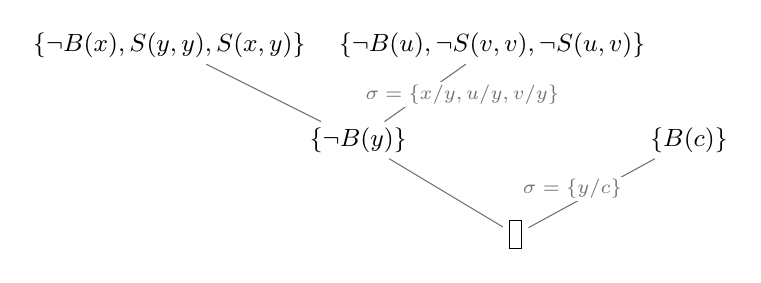
\begin{tikzpicture}[font=\small,every node/.style={inner sep=2pt}]
  \node (c1) at (-3,0) {$\{\neg B(x),S(y,y),S(x,y)\}$};
  \node (c2) at (1.1,0) {$\{\neg B(u),\neg S(v,v),\neg S(u,v)\}$};
  \node (c3) at (3.6,-1.2) {$\{B(c)\}$};
  \node (r1) at (-0.6,-1.2) {$\{\neg B(y)\}$};
  \node (box) at (1.4,-2.4) {$\eclause$};
  \draw[black!55] (c1)--(r1); \draw[black!55] (c2)--(r1);
  \draw[black!55] (r1)--(box); \draw[black!55] (c3)--(box);
  \node[black!55,anchor=west,fill=white,inner sep=1pt] at (-0.55,-0.62) {\scriptsize $\sigma=\{x/y,u/y,v/y\}$};
  \node[black!55,anchor=west,fill=white,inner sep=1pt] at (1.45,-1.82) {\scriptsize $\sigma=\{y/c\}$};
\end{tikzpicture}\obrpopis{Rezoluční zamítnutí holičova paradoxu. Řez $C_1,C_2$ přes dva literály (unifikace $\sigma$ je sjednotí na~$S(y,y)$) dá $\{\neg B(y)\}$; po~řezu s~$\{B(c)\}$ vzniká $\eclause$. U~hran jsou použité unifikace.}
\end{center}
\end{priklad}

\subsection{Hilbertovský kalkulus}

\begin{poznamka}
\emph{Hilbertovský kalkulus} je třetí systém: pevná \textbf{schémata axiomů} (logických tautologií, např.\ $\varphi\to(\psi\to\varphi)$; v~PL navíc $(\forall x)\varphi\to\varphi(x/t)$) a~jediné odvozovací pravidlo \emph{modus ponens} (z~$\varphi$ a~$\varphi\to\psi$ odvoď $\psi$); v~PL ještě pravidlo generalizace. \emph{Důkaz} je posloupnost formulí, každá axiom nebo odvozená z~předchozích. Je korektní a~úplný, ale důkazy se hledají pracně -- hodí se spíš teoreticky. Platí \textbf{věta o~dedukci}: pro sentenci $\varphi$ je $T,\varphi\vdash\psi\iff T\vdash\varphi\to\psi$ (pro formuli s~volnou proměnnou by generalizace větu pokazila).
\end{poznamka}

\subsection{Souhrnná úloha: model teorie}

Následující reálná otázka SZZ propojuje syntaxi (formalizace), sémantiku (model teorie) i~dokazatelnost (hledání modelu vs.\ zamítnutí).

\begin{priklad}[SZZ léto 2024 č.~4: Model teorie] \szzotazka{léto 2024}{4}{Model teorie}\par
\textbf{Zadání.}
\begin{enumerate}[label=(\arabic*)]
  \item Definujte pojmy \emph{struktura jazyka $L=\langle\mathcal R,\mathcal F\rangle$} a~\emph{model teorie $T$}.
  \item V~jazyce $L=\langle Z,S,P\rangle$ (unární predikáty: \uv{složit zkoušku}, \uv{mít štěstí}, \uv{být připraven}) vyjádřete: (a)~\emph{Ne každý, kdo složí zkoušku, má štěstí, ale kdo má štěstí, zkoušku složí.} (b)~\emph{Štěstí přeje připraveným. (Kdo je připraven, má štěstí.)} (c)~\emph{Nějaký student byl připraven, ale zkoušku nesložil.}
  \item Pro $T_1=\{\varphi_1,\varphi_2\}$ a~$T_2=\{\varphi_1,\varphi_2,\varphi_3\}$ najděte model, nebo formálně dokažte, že žádný nemá.
\end{enumerate}

\smallskip
\textbf{Řešení.}
\begin{enumerate}[label=(\arabic*)]
  \item \emph{Struktura} $\mathcal A=\langle A,\mathcal R^{\mathcal A},\mathcal F^{\mathcal A}\rangle$ je neprázdná doména $A$ s~realizacemi: $R^{\mathcal A}\subseteq A^{\mathrm{ar}(R)}$ pro každý relační symbol a~$f^{\mathcal A}\colon A^{\mathrm{ar}(f)}\to A$ pro každý funkční symbol (konstanta $c^{\mathcal A}\in A$). \emph{Model teorie $T$} je struktura, v~níž platí všechny axiomy $T$.
  \item Přirozená formalizace:
    \[
    \varphi_1:\ \neg(\forall x)(Z(x)\to S(x))\ \wedge\ (\forall x)(S(x)\to Z(x)),
    \]
    \[
    \varphi_2:\ (\forall x)(P(x)\to S(x)),\qquad
    \varphi_3:\ (\exists x)\big(P(x)\wedge\neg Z(x)\big),
    \]
    kde (dle zadání) $Z$ značí \uv{složit zkoušku}, $S$ \uv{mít štěstí}, $P$ \uv{být připraven}.
  \item \emph{$T_1$ má model:} jednoprvková doména $A=\{0\}$ s~$Z^{\mathcal A}=\{0\}$, $S^{\mathcal A}=P^{\mathcal A}=\emptyset$. Ověření: $\varphi_2$ platí (nikdo není připraven), $\varphi_1$ platí, protože $(\forall x)(S(x)\to Z(x))$ je vakuózně pravdivé a~$\neg(\forall x)(Z(x)\to S(x))$ platí, neboť $0\in Z$, $0\notin S$.\par
    \emph{$T_2$ model nemá:} z~$\varphi_3$ je nějaký $a$ připraven a~nesložil ($P(a)$, $\neg Z(a)$). Z~$\varphi_2$ pak $S(a)$, z~druhé části $\varphi_1$ (tj.\ $S(a)\to Z(a)$) dostáváme $Z(a)$ -- spor s~$\neg Z(a)$. \emph{Formálně} převedeme $T_2$ na~klauzule (skolemizace $+$ CNF): z~$\varphi_3=(\exists x)(P(x)\wedge\neg Z(x))$ skolemizací (existenční svědek -- konstanta $a$) vzniknou $\{P(a)\}$ a~$\{\neg Z(a)\}$; z~$\varphi_2$ klauzule $\{\neg P(x),S(x)\}$ a~z~druhé části $\varphi_1$, tj.\ $(\forall x)(S(x)\to Z(x))$, po~přejmenování proměnné klauzule $\{\neg S(y),Z(y)\}$. První část $\varphi_1$ dá skolemizací (další konstanta $b$) klauzule $\{Z(b)\}$, $\{\neg S(b)\}$, ty ale k~zamítnutí nepotřebujeme. Rezolucí (strom níže) odvodíme $\eclause$, takže $T_2$ nemá model.
\end{enumerate}

\smallskip
\begin{center}
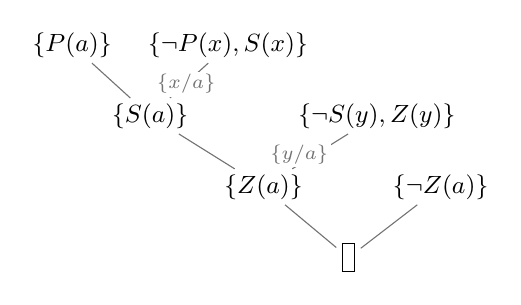
\begin{tikzpicture}[scale=0.9,font=\small,every node/.style={inner sep=1.8pt}]
  \node (p1) at (-3,0) {$\{P(a)\}$};
  \node (c1) at (-0.8,0) {$\{\neg P(x),S(x)\}$};
  \node (s)  at (-1.9,-1) {$\{S(a)\}$};
  \node (c2) at (1.3,-1) {$\{\neg S(y),Z(y)\}$};
  \node (z)  at (-0.3,-2) {$\{Z(a)\}$};
  \node (c3) at (2.2,-2) {$\{\neg Z(a)\}$};
  \node (bx) at (0.9,-3) {$\eclause$};
  \draw[black!55] (p1)--(s); \draw[black!55] (c1)--(s);
  \draw[black!55] (s)--(z); \draw[black!55] (c2)--(z);
  \draw[black!55] (z)--(bx); \draw[black!55] (c3)--(bx);
  \node[black!55,font=\scriptsize,anchor=west,fill=white,inner sep=1pt] at (-1.85,-0.55) {$\{x/a\}$};
  \node[black!55,font=\scriptsize,anchor=west,fill=white,inner sep=1pt] at (-0.25,-1.55) {$\{y/a\}$};
\end{tikzpicture}\\[0.3mm]
{\footnotesize Rezoluční zamítnutí $T_2$ (svědek $a$ z~$\varphi_3$): řezy s~unifikacemi $\{x/a\},\{y/a\}$ vedou k~$\eclause$, takže $T_2$ nemá model.}
\end{center}
\end{priklad}

% ============================================================
\section{Věty o kompaktnosti a úplnosti}

Metavěty spojují obě patra logiky: \emph{korektnost} a~\emph{úplnost} ztotožní dokazatelnost s~platností, \emph{kompaktnost} a~\emph{Löwenheim-Skolemova} věta jsou jejich silné důsledky. U~všech stačí znát znění a~význam.

\subsection{Korektnost a úplnost}

\begin{veta}[O korektnosti a úplnosti]
Tablo metoda i~rezoluce jsou \emph{korektní} a~\emph{úplné}: pro každou (spočetnou) teorii $T$ a~sentenci $\varphi$ platí
\[
T\vdash\varphi\quad\Longleftrightarrow\quad T\models\varphi.
\]
(Pro rezoluci ve~tvaru: množina klauzulí je \emph{nesplnitelná} právě tehdy, když je \emph{rezolucí zamítnutelná}.)
\end{veta}

\begin{intuice}
\textbf{Korektnost} ($\vdash\,\Rightarrow\,\models$) je \uv{bezpečnost}: co dokážeme, opravdu platí (sporné tablo nemůže mít model). \textbf{Úplnost} ($\models\,\Rightarrow\,\vdash$) je \uv{síla}: každou platnou věc kalkulus dokáže (z~dokončené bezesporné větve bychom jinak sestrojili \emph{kanonický model} -- protipříklad). Dohromady je dokazatelnost přesně platnost: syntaxe a~sémantika \uv{vidí totéž} (viz obrázek).
\end{intuice}

\begin{center}
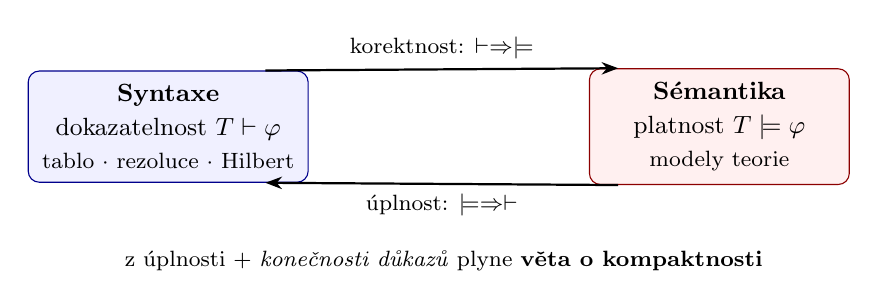
\begin{tikzpicture}[font=\small,
  box/.style={draw,rounded corners,align=center,inner sep=5pt,minimum height=14mm,minimum width=33mm}]
  \node[box,fill=blue!6,draw=blue!55!black] (syn) at (0,0)
    {\textbf{Syntaxe}\\[1pt] dokazatelnost $T\vdash\varphi$\\[1pt] {\footnotesize tablo $\cdot$ rezoluce $\cdot$ Hilbert}};
  \node[box,fill=red!6,draw=red!55!black] (sem) at (7,0)
    {\textbf{Sémantika}\\[1pt] platnost $T\models\varphi$\\[1pt] {\footnotesize modely teorie}};
  \draw[-{Stealth[length=6pt]},thick] (syn.30) -- node[above,font=\footnotesize]{korektnost: $\vdash\Rightarrow\models$} (sem.150);
  \draw[-{Stealth[length=6pt]},thick] (sem.210) -- node[below,font=\footnotesize]{úplnost: $\models\Rightarrow\vdash$} (syn.330);
  \node[align=center] at (3.5,-1.7) {\footnotesize z~úplnosti $+$ \emph{konečnosti důkazů} plyne \textbf{věta o~kompaktnosti}};
\end{tikzpicture}\obrpopis{Korektnost a~úplnost ztotožňují dokazatelnost ($\vdash$) s~platností ($\models$). Tablo důkaz je vždy \emph{konečný}, použije tedy jen konečně mnoho axiomů -- odtud kompaktnost.}
\end{center}

\begin{poznamka}
\textbf{\uv{Úplnost} a~\uv{kompletnost} nezaměňovat.} \emph{Úplnost kalkulu} je vlastnost \emph{dokazovacího systému}: $T\models\varphi\Rightarrow T\vdash\varphi$ (co platí, umíme dokázat). \emph{Kompletní teorie} je vlastnost \emph{teorie}: o~každé sentenci rozhodne -- je v~ní pravdivá, nebo lživá (žádná otevřená otázka; viz sekci~6). Jsou to různé pojmy s~matoucně podobnými názvy. Pozor zvlášť na~Gödela: \uv{věta o~ne\emph{úplnosti}} (sekce~6) říká, že dostatečně silná teorie \emph{není kompletní} -- popírá tedy \emph{kompletnost teorie}, nikoli úplnost kalkulu (ta platí dál).
\end{poznamka}

\subsection{Věta o kompaktnosti}

\begin{veta}[O kompaktnosti (výrokové i predikátové logiky)]
Teorie má model právě tehdy, když má model \emph{každá její konečná část}.
\end{veta}

\begin{intuice}
Jedna implikace je triviální (model celku je modelem každé části). Druhá je obsahem věty: \emph{lokální} splnitelnost (po~konečných kouscích) vynutí \emph{globální}. Důvod (náčrt): nemá-li $T$ model, je sporná, tedy $T\vdash\eclause$ (úplnost); ale důkaz je \emph{konečný} a~použije jen konečně mnoho axiomů $T'\subseteq T$ -- a~už ta konečná $T'$ je sporná. Kompaktnost je most mezi konečným a~nekonečným.
\end{intuice}

\begin{priklad}[Použití kompaktnosti]
\textbf{Zadání.}\par
Ukažte, že (spočetně) nekonečný graf $G$ je bipartitní (2-obarvitelný), právě když je bipartitní \emph{každý jeho konečný podgraf}.

\smallskip
\textbf{Řešení.} Pro každý vrchol $v$ vezměme prvovýrok $p_v$ (\uv{$v$ má barvu 1}) a~teorii
\[
T=\{\,p_u\leftrightarrow\neg p_v\ :\ \{u,v\}\in E(G)\,\}
\]
(\uv{sousedé mají různé barvy}). Modely $T$ odpovídají dvojobarvením $G$, tedy $G$ je bipartitní právě tehdy, když má $T$ model. Podle kompaktnosti stačí, aby měla model \emph{každá konečná} $T'\subseteq T$. Taková $T'$ mluví o~konečně mnoha hranách, tj.\ o~konečném podgrafu $G'$; ten je z~předpokladu bipartitní, a~jeho obarvení je modelem $T'$. Tedy $T$ má model a~$G$ je bipartitní. \emph{(Stejnou šablonou se dokáže $k$-obarvitelnost nebo rozšíření částečného uspořádání na~lineární.)}
\end{priklad}

\begin{intuice}
Druhá slavná aplikace: k~$\mathrm{Th}(\mathbb{N})$ (všem pravdivým sentencím standardní aritmetiky) přidáme konstantu $c$ a~axiomy $\underline n<c$ pro všechna $n$. Každá konečná část má model ($c$ = dost velké číslo), takže podle kompaktnosti má model i~celek -- \emph{nestandardní model} aritmetiky s~prvkem větším než všechna \uv{obyčejná} čísla.
\end{intuice}

\subsection{Löwenheim-Skolemova věta}

\begin{veta}[Löwenheim-Skolem]
Každá bezesporná teorie ve~spočetném jazyce má \emph{spočetný} model (bez~rovnosti spočetně nekonečný; s~rovností konečný nebo spočetně nekonečný).
\end{veta}

\begin{intuice}
Plyne z~úplnosti: dokončené bezesporné tablo dá kanonický model, jehož doménou jsou konstantní termy -- a~těch je jen spočetně. Důsledek je překvapivý: i~teorie \uv{velkých} struktur (např.\ reálných čísel) má spočetný model. Odtud plyne existence elementárně ekvivalentních, ale neizomorfních struktur: $\mathrm{Th}(\langle\mathbb{R},\le\rangle)$ má spočetný model, a~ten s~nespočetnou $\langle\mathbb{R},\le\rangle$ izomorfní být nemůže (konkrétně $\langle\mathbb{Q},\le\rangle\equiv\langle\mathbb{R},\le\rangle$, viz DeLO v~sekci~6).
\end{intuice}

% ============================================================
\section{Rozhodnutelnost}

Poslední otázka je algoritmická: umíme pro danou teorii \emph{strojově} rozhodnout, co z~ní plyne? Klíčem je pojem \emph{kompletní} teorie a~jeho vztah k~rozhodnutelnosti.

\subsection{Kompletní teorie a kritéria kompletnosti}

\begin{definice}[Kompletní teorie, elementární ekvivalence]
Struktury $\mathcal A,\mathcal B$ jsou \emph{elementárně ekvivalentní} ($\mathcal A\equiv\mathcal B$), platí-li v~nich tytéž sentence. Teorie $T$ je \emph{kompletní}, je-li bezesporná a~každá sentence je v~ní pravdivá, nebo lživá (táž definice jako ve~výrokové logice, sekce~2). Ekvivalentně: $T$ je kompletní \emph{právě tehdy, když má jediný model až na~elementární ekvivalenci}.
\end{definice}

\begin{intuice}
Kompletní teorie \uv{úplně popisuje} svůj typ struktury -- o~žádné sentenci nenechává otázku otevřenou. Pozor: na~rozdíl od~výrokové logiky to \emph{neznamená} jediný model (jeden model má vždy nekonečně mnoho izomorfních kopií), jen jedinou \emph{teorii struktury} $\mathrm{Th}(\mathcal A)$.
\end{intuice}

\begin{veta}[Kritérium kompletnosti přes $\omega$-kategoricitu]
Je-li teorie $T$ ve~spočetném jazyce \emph{$\omega$-kategorická} (má až na~izomorfismus jediný spočetně nekonečný model) a~je-li jazyk bez rovnosti, nebo $T$ nemá konečné modely, pak je $T$ \emph{kompletní}.
\end{veta}

\begin{intuice}
Myšlenka: podle Löwenheim-Skolemovy věty je každý model $T$ elementárně ekvivalentní nějakému spočetně nekonečnému modelu (bez rovnosti vždy, s~rovností pro nekonečné modely -- proto předpoklad, že konečné modely nejsou). Ten je ale podle $\omega$-kategoricity až na~izomorfismus jediný, takže jsou \emph{všechny} modely $T$ navzájem elementárně ekvivalentní -- a~to je kompletnost. Příklad: \textbf{DeLO} (hustá lineární uspořádání bez~konců, jako $\langle\mathbb{Q},\le\rangle$) je $\omega$-kategorická (metoda \uv{cik-cak}), tedy \emph{kompletní}; teorie tak rozhodne každou sentenci o~hustých lineárních uspořádáních bez konců.
\end{intuice}

\subsection{Rozhodnutelnost a její vztah ke kompletnosti}

\begin{definice}[Rozhodnutelná teorie]
Teorie $T$ je \emph{rozhodnutelná}, existuje-li algoritmus, který pro každou vstupní sentenci $\varphi$ doběhne a~odpoví, zda $T\models\varphi$. Je \emph{rekurzivně axiomatizovaná}, lze-li algoritmicky rozpoznat, které formule jsou její axiomy.
\end{definice}

\begin{veta}[Kompletnost dává rozhodnutelnost]
Bezesporná \emph{rekurzivně axiomatizovaná} a~\emph{kompletní} teorie je \emph{rozhodnutelná}.
\end{veta}

\begin{intuice}
Algoritmus: pro vstup $\varphi$ konstruujeme \emph{paralelně} systematické tablo důkazy pro $\varphi$ (tablo s~$F\varphi$) a~pro $\neg\varphi$ (tablo s~$T\varphi$). Z~kompletnosti je dokazatelná právě jedna z~nich, a~díky korektnosti+úplnosti a~konečnosti důkazů se příslušné tablo po~konečně mnoha krocích uzavře -- algoritmus tak vždy doběhne a~odpoví. (Sama rekurzivní axiomatizace dává jen \emph{částečnou} rozhodnutelnost; teprve kompletnost zaručí, že se dočkáme i~záporné odpovědi.)
\end{intuice}

\subsection{Příklady rozhodnutelných a nerozhodnutelných teorií}

\begin{center}
\renewcommand{\arraystretch}{1.15}
\begin{tabular}{p{0.46\linewidth} p{0.46\linewidth}}
\toprule
\textbf{Rozhodnutelné} & \textbf{Nerozhodnutelné}\\
\midrule
hustá lineární uspořádání (DeLO) & \textbf{predikátová logika} obecně (Churchova věta)\\
Presburgerova aritmetika $\mathrm{Th}(\langle\mathbb{N},S,+,0\rangle)$ & plná aritmetika $\mathrm{Th}(\mathbb{N})$ (s~$+$ i~$\cdot$)\\
algebraicky uzavřená tělesa & Robinsonova/Peanova aritmetika\\
reálně uzavřená tělesa (i~euklidovská geometrie) & Hilbertův 10.\ problém (diofantické rovnice; problém, ne teorie)\\
teorie konečné struktury (v~konečném jazyce) & teorie grup, ZFC\\
\bottomrule
\end{tabular}
\end{center}

\begin{veta}[Churchova věta]
Predikátová logika je \emph{nerozhodnutelná}: neexistuje algoritmus, který by pro každou vstupní formuli (v~libovolném jazyce, ten je součástí vstupu) rozhodl, zda je logicky platná ($\models\varphi$).
\end{veta}

\begin{intuice}
Dokazuje se \emph{redukcí} z~nerozhodnutelného problému (existence přirozeného řešení diofantické rovnice, Hilbertův 10.\ problém): pro sentenci $\varphi=(\exists\bar x)\,p(\bar x)=q(\bar x)$ platí $\mathbb{N}\models\varphi\iff{}\models\psi_Q\to\varphi$, kde $\psi_Q$ je konjunkce (konečně mnoha) axiomů Robinsonovy aritmetiky~$Q$. Algoritmus na~platnost by tedy rozhodl i~Hilbertův problém. Nerozhodnutelnost je vlastnost \emph{obecného} případu: v~jazyce jen s~unárními relačními symboly (bez funkčních) je platnost rozhodnutelná. Predikátová logika je ovšem \emph{částečně} rozhodnutelná (je-li $\models\varphi$, tablo to po~konečně krocích potvrdí) -- jen u~neplatných formulí výpočet nemusí skončit.
\end{intuice}

\begin{veta}[Gödelovy věty o neúplnosti]
\emph{(1.\ věta)} Každá bezesporná rekurzivně axiomatizovaná teorie obsahující \uv{dostatek aritmetiky} (Robinsonovu aritmetiku), jejímž modelem je standardní $\mathbb{N}$, je \emph{neúplná}, tj.\ \emph{není kompletní}: existuje sentence pravdivá v~$\mathbb{N}$, kterou teorie nedokáže ani nevyvrátí. \emph{(2.\ věta)} Je-li navíc dostatečně silná (postačí extenze Peanovy aritmetiky), nedokáže (zformalizovanou) \emph{vlastní bezespornost}.
\end{veta}

\begin{intuice}
Aritmetika přirozených čísel je principiálně \uv{příliš bohatá} na~úplné efektivní zachycení: pravdivost v~$\mathbb{N}$ \emph{nelze} ztotožnit s~dokazatelností v~žádné rozumné teorii. Proto $\mathrm{Th}(\mathbb{N})$ ani není rekurzivně axiomatizovatelná, a~je \emph{nerozhodnutelná}. (Důkazy -- diagonalizace, aritmetizace syntaxe -- jsou nad~rámec M6; stačí znát znění a~smysl.)
\end{intuice}

% ============================================================
\section*{Shrnutí}
\addcontentsline{toc}{section}{Shrnutí}

\begin{poznamka}
\textbf{Klíčové vlastnosti a vzorce (přehled k~SZZ).} Stručný výčet klíčových definic, vět a vzorců okruhu M6. Zkratky: VL~$=$~výroková logika, PL~$=$~predikátová logika prvního řádu, mgu~$=$~nejobecnější unifikátor.

\smallskip
\emph{Syntaxe VL a~PL.}
\begin{itemize}
  \item VL: jazyk $=$ neprázdná množina prvovýroků $\mathbb{P}$; formule induktivně ($p\in\mathbb{P}$; $\neg\varphi$; $\varphi\conn\psi$); \emph{strom výroku} $=$ strukturální analýza; \emph{podvýrok} $=$ podstrom.
  \item PL: jazyk dán signaturou $\langle\mathcal R,\mathcal F\rangle$ (relační a funkční symboly s~aritami; konstanta $=$ nulární funkce). \emph{Termy} induktivně (proměnné, konstanty, $f(t_1,\dots,t_n)$). \emph{Formule}: atomy $R(\bar t)$ nebo $=$, pak $\neg$, $\conn$, $(\forall x)\varphi$, $(\exists x)\varphi$.
  \item Výskyt proměnné $x$ je \emph{vázaný} uvnitř $(\forall x)\psi$ nebo $(\exists x)\psi$, jinak \emph{volný}. \emph{Otevřená} formule $=$ bez kvantifikátoru; \emph{uzavřená} (\emph{sentence}) $=$ bez volné proměnné. Sentence má hodnotu nezávisle na~ohodnocení.
  \item \emph{Instance} $\varphi(x/t)$: nahraď volné výskyty $x$ termem $t$ (podmínka substituovatelnosti: $t$ nesmí zachytit volnou proměnnou). \emph{Varianta}: přejmenuj vázanou proměnnou (bezpečná příprava před dosazením).
  \item \emph{Struktura} $\mathcal A=\langle A,\mathcal R^{\mathcal A},\mathcal F^{\mathcal A}\rangle$: neprázdná doména $A$; pro $n$-ární $R$: realizace $R^{\mathcal A}\subseteq A^n$; pro $n$-ární $f$: $f^{\mathcal A}\colon A^n\to A$ (konstanta $c^{\mathcal A}\in A$). \emph{Model teorie} $T=$ struktura, v~níž platí všechny axiomy.
\end{itemize}

\smallskip
\emph{Normální formy (CNF, DNF, PNF) a~skolemizace.}
\begin{itemize}
  \item \emph{Literál} $=$ $p$ nebo $\neg p$; \emph{klauzule} $=$ disjunkce literálů; \emph{elementární konjunkce} $=$ konjunkce literálů. \textbf{CNF} $=$ konjunkce klauzulí; \textbf{DNF} $=$ disjunkce elem.\ konjunkcí; existují vždy ke~každé formuli.
  \item Převod \textbf{sémanticky}: DNF $=$ jedna elem.\ konjunkce na~každý \emph{model} ($p^{v(p)}$); CNF $=$ jedna klauzule na~každý \emph{nemodel} ($p^{1-v(p)}$). Převod \textbf{úpravami}: eliminuj $\leftrightarrow$, $\to$; zatlač $\neg$ k~listům (de~Morgan); distribuuj.
  \item Prázdná klauzule $\eclause$ je nesplnitelná; prázdná elem.\ konjunkce je tautologie. CNF tautologie $\iff$ každá klauzule obsahuje opačné literály; DNF splnitelné $\iff$ $\exists$ elem.\ konjunkce bez opačných literálů. CNF je vstupem \textbf{SAT} (NP-úplné; řeší se rezolucí nebo DPLL).
  \item \textbf{PNF} (prenexní): tvar $(Q_1x_1)\cdots(Q_nx_n)\,\varphi'$, kde $Q_i\in\{\forall,\exists\}$ a~$\varphi'$ otevřená. Postup: eliminuj $\leftrightarrow$, $\to$; flip $\neg Q\sim\overline{Q}\neg$; vytahuj kvantifikátory ven. \textbf{Klíčová past:} $\forall$ v~antecedentu implikace se překlopí na~$\exists$ ($((\forall x)\varphi)\to\psi\sim(\exists x)(\varphi\to\psi)$).
  \item \textbf{Skolemizace}: sentence $\to$ PNF $\to$ nahraď každé $(\exists y)$ (před nímž stojí $\forall x_1,\dots,\forall x_m$) novým $m$-árním funkčním symbolem $f(x_1,\dots,x_m)$ ($m{=}0$: konstanta) $\to$ vypusť zbylé $\forall$. Výsledek je \emph{ekvisplnitelná} otevřená teorie (ne ekvivalentní); nutno skolemizovat ze~sentence.
\end{itemize}

\smallskip
\emph{Sémantika: model, platnost, důsledek.}
\begin{itemize}
  \item VL: ohodnocení $v\colon\mathbb{P}\to\{0,1\}$, hodnota výroku rekurzivně po~stromu; $v\models\varphi$, $\Mset(\varphi)$, $\Mset(T)=\bigcap\Mset(\varphi_i)$. PL: Tarskiho rekurze -- $\mathrm{H}^{\mathcal A}((\forall x)\varphi)[e]=\min_{a\in A}\mathrm{H}^{\mathcal A}(\varphi)[e(x/a)]$; $\exists$ je $\max$.
  \item \textbf{Tautologie} $\models\varphi$: $\Mset(\varphi)=\Mset_{\mathbb{P}}$; \textbf{sporný}: $\Mset(\varphi)=\emptyset$; \textbf{nezávislý}: vlastní neprázdná část; \textbf{splnitelný}: $\Mset(\varphi)\neq\emptyset$. Kategorie jsou vzájemně výlučné (vyjma splnitelnost).
  \item \textbf{Důsledek} $T\models\varphi$: $\Mset(T)\subseteq\Mset(\varphi)$ (každý model $T$ je modelem $\varphi$). \textbf{Klíčová ekvivalence:} $T\models\varphi\iff T\cup\{\neg\varphi\}$ nemá model -- základ důkazů sporem (tablo, rezoluce).
  \item Analýza teorie nad $|\mathbb{P}|=n$: celkem $2^n$ ohodnocení; teorie s~$k$ modely má $(2^k{-}2)\cdot 2^{2^n-k}$ nezávislých výroků (libovolná volba na~$2^n-k$ ohodnoceních mimo $\Mset(T)$, netriviální na~$k$ modelech $T$).
  \item \emph{Kompletní teorie} $=$ bezesporná a~bez nezávislé sentence. VL: právě tehdy, když má \emph{jediný} model; PL: jediný model až na~\emph{elementární ekvivalenci} ($\mathcal A\equiv\mathcal B$: tytéž sentence).
\end{itemize}

\smallskip
\emph{Extenze teorií.}
\begin{itemize}
  \item Extenze $T'$ teorie $T$ (jazyk $L\subseteq L'$): $\Csq_L(T)\subseteq\Csq_{L'}(T')$; pro jednoduché extenze ($L'=L$) ekvivalentní $\Mset(T')\subseteq\Mset(T)$ (více axiomů $=$ méně modelů $=$ silnější teorie).
  \item \emph{Konzervativní} extenze: o~původním jazyce $L$ nedokáže nic nového. \emph{Extenze o~definice} je vždy konzervativní (každý model $T$ se na~model $T'$ expanduje jednoznačně): relační $R(\bar x)\leftrightarrow\psi(\bar x)$; funkční: nutno axiom existence a~jednoznačnosti $\psi$ v~$T$.
  \item \emph{Ekvisplnitelnost}: $T$ a~$T'$ (různé jazyky) mají model oba, nebo žádný. Skolemizace $\Rightarrow$ ekvisplnitelná (ne ekvivalentní) extenze; stačí pro důkaz sporem.
\end{itemize}

\smallskip
\emph{Dokazatelnost: tablo, rezoluce, Hilbert.}
\begin{itemize}
  \item Obecné schéma: $T\vdash\varphi$ dokažeme sporem -- sporujeme $T\cup\{\neg\varphi\}$ (kořen tabla $F\varphi$; vstup rezoluce $T\cup\{\neg\varphi\}$ v~CNF).
  \item \textbf{Tablo VL}: položky $T\psi$/$F\psi$; atomická tabla: $T\wedge$: oba pod sebou; $F\wedge$: větví; $T\vee$: větví; $F\vee$: oba; $T{\to}$: větví ($F\varphi\mid T\psi$); $F{\to}$: $T\varphi,F\psi$; $T\neg$: $F\varphi$; $F\neg$: $T\varphi$. Sporná větev \closed{}: $T\psi$ a~$F\psi$ na~téže větvi. Dokončená bezesporná větev $\Rightarrow$ kanonický model $v(p)=1 \iff Tp$ na~větvi.
  \item \textbf{Tablo PL}: tytéž spojkové rozvoje $+$ kvantifikátorová pravidla -- \uv{svědek} ($T(\exists x)\varphi\rightsquigarrow T\varphi(x/c)$, $F(\forall x)\varphi\rightsquigarrow F\varphi(x/c)$, kde $c$ nový): přidáme konstantu pro existenci; \uv{všichni} ($T(\forall x)\varphi\rightsquigarrow T\varphi(x/t)$ pro libovolný term $t$, $F(\exists x)\varphi\rightsquigarrow F\varphi(x/t)$): položka zůstává \uv{nehotová}, opakuje se. Jazyk s~rovností: přidej axiomy rovnosti.
  \item \textbf{Rezoluce VL}: CNF v~množinové repr.; rezolventa $C_1,C_2$ přes literál $\ell$: $(C_1\setminus\{\ell\})\cup(C_2\setminus\{\overline{\ell}\})$; zamítnutí $=$ odvození $\eclause$; nesplnitelná $\iff$ zamítnutelná. Řez vždy jen přes jednu dvojici opačných literálů (ne přes dvě zároveň).
  \item \textbf{Rezoluce PL}: skolemizace $+$ CNF $\to$ přejmenuj proměnné klauzulí na~disjunktní $\to$ najdi mgu řezaných literálů (occurs-check: $x$ nelze unifikovat s~$f(x)$) $\to$ rezolventa $=$ zbytky po~aplikaci mgu.
  \item \textbf{Hilbert}: schémata logických tautologií jako axiomů $+$ modus ponens; v~PL navíc generalizace. Věta o~dedukci (pro sentenci $\varphi$): $T,\varphi\vdash\psi\iff T\vdash\varphi\to\psi$. Spíše teoretický nástroj.
\end{itemize}

\smallskip
\emph{Věty o korektnosti, úplnosti a kompaktnosti.}
\begin{itemize}
  \item \textbf{Korektnost} ($\vdash\Rightarrow\models$): co je dokazatelné, platí. \textbf{Úplnost} ($\models\Rightarrow\vdash$): co platí, je dokazatelné. Dohromady $T\vdash\varphi\iff T\models\varphi$. Pro rezoluci: $S$ nesplnitelná $\iff$ $S$ rezolucí zamítnutelná.
  \item \textbf{Pozor na záměnu}: \emph{úplnost kalkulu} ($\models\Rightarrow\vdash$, vlastnost dokazovacího systému) $\neq$ \emph{kompletnost teorie} (o~každé sentenci rozhodne, vlastnost teorie). Gödelova věta o~\emph{ne}úplnosti mluví o~\emph{nekompletnosti teorie}, ne o~kalkulu.
  \item \textbf{Kompaktnost}: $T$ má model $\iff$ každá konečná $T'\subseteq T$ má model. Plyne z~úplnosti (důkaz je konečný $\Rightarrow$ použije jen konečně mnoho axiomů). Aplikace: nekonečný graf bipartitní $\iff$ každý konečný podgraf bipartitní; existence nestandardního modelu aritmetiky.
  \item \textbf{Löwenheim-Skolem}: bezesporná teorie ve~spočetném jazyce má spočetný model (bez rovnosti spočetně nekonečný; s~rovností konečný nebo spočetně nekonečný). Překvapivý důsledek: i~teorie reálných čísel má spočetný model.
\end{itemize}

\smallskip
\emph{Rozhodnutelnost.}
\begin{itemize}
  \item Kritérium $\omega$-kategoricity: teorie ve~spočetném jazyce bez~rovnosti (nebo bez~konečných modelů) je \emph{kompletní}, je-li \emph{$\omega$-kategorická} (jediný spočetně nekonečný model až na~$\cong$). Příklad: \textbf{DeLO} (hustá lin.\ uspořádání bez konců, jako $\langle\mathbb{Q},\le\rangle$) -- $\omega$-kategorická, tedy kompletní.
  \item \emph{Rekurzivně axiomatizovaná} $+$ \emph{kompletní} $\Rightarrow$ \emph{rozhodnutelná}: paralelně budujeme tabla pro $\varphi$ a~$\neg\varphi$; kompletnost zaručí, že jedno skončí po~konečně krocích.
  \item \textbf{Rozhodnutelné}: DeLO; Presburgerova aritmetika $\mathrm{Th}(\langle\mathbb{N},S,+,0\rangle)$; algebraicky uzavřená tělesa; reálně uzavřená tělesa; teorie konečné struktury (v~konečném jazyce).
  \item \textbf{Nerozhodnutelné}: predikátová logika (Churchova věta, jazyk je součástí vstupu -- redukce z~Hilbertova 10.~problému; PL je ale \emph{částečně} rozhodnutelná: $\models\varphi$ tablo potvrdí, zápornou odpověď ne); $\mathrm{Th}(\mathbb{N})$ (plná aritmetika s~$+,\cdot$); Robinsonova/Peanova aritmetika.
  \item \textbf{Gödelovy věty o~neúplnosti} (znění): (1.)~každá bezesporná rek.\ axiomatizovaná teorie s~dostatkem aritmetiky (a~s~modelem $\mathbb{N}$) \emph{není kompletní} (existuje sentence pravdivá v~$\mathbb{N}$ bez důkazu i~vyvrácení v~$T$); (2.)~taková teorie nedokáže vlastní bezespornost.
\end{itemize}
\end{poznamka}

\section*{Zdroje}
\addcontentsline{toc}{section}{Zdroje}

{\raggedright
\begin{itemize}
  \item J.~Bulín: \emph{NAIL062 Výroková a predikátová logika: zápisky z~přednášky}, MFF UK, zimní semestr 2025 (primární zdroj výkladu: syntaxe a~sémantika VL i~PL, normální formy, tablo metoda, rezoluce, extenze a~skolemizace, věty o~úplnosti a~kompaktnosti, rozhodnutelnost, Gödelovy věty). Existuje i~anglická verze \emph{Propositional and Predicate Logic: Lecture Notes}.\\ \url{https://github.com/jbulin-mff-uk/nail062}
  \item J.~Bulín: sady příkladů ke cvičení NAIL062 se vzorovými řešeními (kalibrace hloubky řešených příkladů).\\ \url{https://github.com/jbulin-mff-uk/nail062/tree/main/tutorial/priklady}
  \item A.~Nerode, R.~A.~Shore: \emph{Logic for Applications}, 2.~vyd., Springer, 1997, a~M.~Ben-Ari: \emph{Mathematical Logic for Computer Science}, 3.~vyd., Springer, 2012 (učebnice, na~nichž stojí přednáška).
  \item MFF UK: požadavky ke státní závěrečné zkoušce (Informatika, Bc.) a~zadání otázek z~minulých termínů.\\ \url{https://www.mff.cuni.cz/cs/studenti/bakalarske-studium/statni-zaverecne-zkousky/bakalarske-statni-zkousky-studijniho-programu-informatika}
\end{itemize}
\par}

\end{document}
